\chapter{Valutazione sperimentale}
Il presente capitolo illustra il processo di validazione empirica del lavoro svolto. Facendo riferimento alla metodologia di poisoning e alle architetture descritte nel capitolo precedente, vengono qui analizzati nel dettaglio i dataset utilizzati, le metriche adottate per la valutazione dei classificatori e i risultati ottenuti dall'approccio sviluppato.
\section{Descrizione del dataset}
Per la validazione sperimentale sono stati utilizzati due dataset distinti, le cui distribuzioni sono riassunte nella Tabella \ref{tab:ember_dist} e in Tabella \ref{tab:WIPE4ADV_dist}.

Il primo, EMBER \cite{2018arXiv180404637A}, rappresenta un benchmark consolidato per il rilevamento statico di malware. Esso fornisce feature estratte con LIEF da un vasto corpus di 1,1 milioni di file Portable Executable (PE). Per questo studio, è stato utilizzato il sottoinsieme etichettato, che comprende un totale di 800.000 campioni, suddivisi in 600.000 per il training e 200.000 per il test. Come evidenziato nella Tabella \ref{tab:ember_dist}, il dataset è perfettamente bilanciato tra malware e goodware in entrambe le partizioni.

Il secondo dataset, denominato WIPE4ADV\cite{fi16050168}, è stato impiegato per valutare l'efficacia degli attacchi su un diverso modello bersaglio. Sebbene il dataset originale comprenda oltre 27.000 file PE, in questo lavoro è stato selezionato un sottoinsieme specifico di 5.000 file (2.500 per classe). La componente benigna proviene dal repository PEMML\footnote{https://practicalsecurityanalytics.com/pe-malware-machine-learning-dataset/}, con file del biennio 2017-2018, mentre i malware sono stati estratti da VirusShare, focalizzandosi su minacce recenti (2021 e 2023). Questo sottoinsieme è stato partizionato in un training set di 4.000 esempi e un test set di 1.000 esempi, mantenendo il bilanciamento tra le classi, come mostrato nella Tabella \ref{tab:WIPE4ADV_dist}.

\begin{table}[htbp]
    \centering
    \caption{Distribuzione dataset EMBER}
    \label{tab:ember_dist}
    \begin{tabular}{lcc}
        \toprule
        \textbf{Subset} & \textbf{Goodware} & \textbf{Malware} \\
        \midrule
        Training & 300.000 & 300.000 \\
        Test & 100.000 & 100.000 \\
        \midrule
        \textbf{Totale} & \textbf{400.000} & \textbf{400.000} \\
        \bottomrule
    \end{tabular}
\end{table}

\begin{table}[htbp]
    \centering
    \caption{Distribuzione subset dataset WIPE4ADV}
    \label{tab:WIPE4ADV_dist}
    \begin{tabular}{lcc}
        \toprule
        \textbf{Subset} & \textbf{Goodware} & \textbf{Malware} \\
        \midrule
        Training & 2.000 & 2.000 \\
        Test & 500 & 500 \\
        \midrule
        \textbf{Totale} & \textbf{2.500} & \textbf{2.500} \\
        \bottomrule
    \end{tabular}
\end{table}

\section{Metriche di Valutazione}
Per valutare le prestazioni dei modelli di classificazione, sono state utilizzate le metriche standard derivate dalla matrice di confusione, uno strumento che permette di visualizzare le performance di un algoritmo confrontando le classi predette con quelle reali. Gli elementi costitutivi di tale matrice sono i True Positive (TP) e True Negative (TN), che rappresentano rispettivamente i campioni positivi (malware) e negativi (goodware) correttamente classificati, contrapposti ai False Positive (FP) e False Negative (FN), che indicano invece gli errori di classificazione, ovvero campioni negativi etichettati erroneamente come positivi e viceversa.

Sulla base di questi valori, è possibile calcolare diverse metriche di sintesi. L'Accuracy (Accuratezza) rappresenta la frazione di predizioni corrette rispetto al totale dei campioni esaminati ed è definita come:
\begin{equation}
    Accuracy = \frac{TP + TN}{TP + TN + FP + FN}
\end{equation}
In questo lavoro, si farà riferimento in particolare alla \textit{Overall Accuracy}, calcolata sull'intero test set.

Per analizzare più in dettaglio le performance, le metriche sono state calcolate separatamente per ciascuna classe (Goodware e Malware), considerando di volta in volta la classe in esame come ``positiva''. La Precision (Precisione) indica l'affidabilità del classificatore nel predire una specifica classe, ed è calcolata come il rapporto tra i veri positivi per quella classe e il totale dei campioni predetti come appartenenti ad essa:
\begin{equation}
    Precision = \frac{TP}{TP + FP}
\end{equation}
La Recall (Richiamo), invece, misura la capacità del classificatore di individuare tutti i campioni appartenenti a una data classe, ed è data dal rapporto tra i veri positivi e il totale dei campioni reali di quella classe:
\begin{equation}
    Recall = \frac{TP}{TP + FN}
\end{equation}

Infine, per ottenere una valutazione bilanciata che tenga conto di entrambe le metriche precedenti, si utilizza l'F1-Score, definito come la media armonica tra Precision e Recall:
\begin{equation}
    F1 = 2 \cdot \frac{Precision \cdot Recall}{Precision + Recall}
\end{equation}
Nel seguito verranno riportati i valori di queste metriche distinti per ciascuna classe, al fine di evidenziare l'effetto del poisoning sul modello, nella individuazione della classe Goodware.

\section{Dettagli implementativi}
Il codice per lo studio sperimentale è stato sviluppato in Python 3.6, utilizzando PyTorch come framework per le reti neurali. Per l'estrazione delle feature è stata impiegata la libreria LIEF (versione 0.9), mentre per gli attacchi adversarial: per GAMMA si è fatto uso di secml-malware nella versione 0.2.4.1,invece per OLIVANDER la versione piu recente disponibile su Github.

Per quanto riguarda le architetture valutate, la DNN implementata è costituita da tre layer Fully Connected (FC) con, rispettivamente, 512, 128 e 8 neuroni, seguiti da un layer di output a 2 neuroni. In questa architettura, sono stati inseriti due layer di Batch Normalization: uno precedente al primo layer FC e uno posizionato tra il secondo e il terzo. La funzione di attivazione Tanh è stata applicata a tutti i layer interni, mentre per l'ultimo layer è stata utilizzata la funzione Softmax per ottenere le probabilità di output.

Il modello MalConv, invece, è una rete neurale convoluzionale, Il flusso di elaborazione inizia con la mappatura della sequenza di byte in ingresso (incluso un token di padding) in uno spazio vettoriale tramite un layer di embedding addestrabile, che proietta ogni byte in un vettore denso di dimensione 8. A questo segue un blocco di convoluzione unidimensionale con 128 filtri, caratterizzati da kernel e stride di dimensione 500, che utilizza una funzione di attivazione \textit{gated} definita come \(G_0 = A \otimes \sigma(B)\). L'output convoluzionale viene ridotto da un layer di \textit{temporal max-pooling} globale, che estrae il valore massimo per ogni canale, producendo un singolo vettore di feature. Questo vettore alimenta infine un layer FC da 128 unità e un layer Softmax finale per la classificazione.

il modello MalConv utilizzato è fornito dal team EMBER\footnote{https://github.com/elastic/ember/tree/master/malconv},l'implementazione differisce dalla paper originale per la limitazione della sequenza di byte di ingresso ad 1 MB.

Sia il modello MalConv che la DNN(successivamente chiamata \(DNN_{ember}\)) sono stati addestrati sul dataset EMBER,mentre la \(DNN_{target}\) è addestrata sul subset del dataset WIPE4ADV

Sia GAMMA che OLIVANDER sono stati originariamente progettati per evadere un modello in maniera tale che esempi malware siano etichettati come goodware. Nel caso di GAMMA, per invertire l'obiettivo dell'attacco,l'adattamento è stato facilitato dato l'utilizzo del toolkit DEAP: è bastato impostare un peso negativo per la funzione di fitness. In tal modo, l'algoritmo genetico non premia più l'individuo con la minore probabilità di essere classificato come malware, bensì quello con la probabilità maggiore. Per OLIVANDER, invece, sono state necessarie modifiche strutturali al codice: è stata alterata la logica di selezione dei campioni per processare i file classificati come goodware (classe 0) e la condizione di terminazione è stata invertita per considerare un successo la classificazione come malware (classe 1).

Gli algoritmi GAMMA e OLIVANDER sono stati eseguiti con i parametri consigliati di default nella configurazione che usa l'injection, cioè il payload adversarial viene aggiunto come una nuova sezione nel file Windows PE , come modifica che preserva la funzionalità.


\section{Analisi ed interpretazione dei risultati}

In questa sezione vengono discussi i risultati sperimentali ottenuti. 
Inizialmente, viene valutata la performance del modello bersaglio \(DNN_{target}\) sul test set di WIPE4ADV, che funge da baseline per le successive analisi. La Figura~\ref{fig:dnn_test_confusion} mostra la matrice di confusione ottenuta.

\begin{figure}[htbp]
    \centering
    \includegraphics[width=0.5\textwidth]{images/dnn4000test.png}
    \caption{Matrice di confusione di \(DNN_{target}\) sul Test Set}
    \label{fig:dnn_test_confusion}
\end{figure}

Successivamente, è importante quantificare i TN dei modelli surrogati sul training set di WIPE4ADV, in quanto essi costituiscono la base di partenza per la generazione degli attacchi.
Il modello \(MalConv\) ha classificato correttamente 1.965 campioni su 2.000, mentre il modello \(DNN_{ember}\) ne ha classificati correttamente 1.588. Questi numeri rappresentano il totale dei tentativi di attacco effettuati, da cui derivano le percentuali di successo riportate successivamente.
La Figura~\ref{fig:surrogate_train_confusion} riporta le matrici di confusione per i due modelli surrogati sul training set.

\begin{figure}[htbp]
    \centering
    \begin{subfigure}[b]{0.45\textwidth}
        \centering
        \includegraphics[width=\textwidth]{images/malconvTrainSet.png}
        \caption{\(MalConv\) (Train)}
        \label{fig:malconvtrain}
    \end{subfigure}
    \hfill
    \begin{subfigure}[b]{0.45\textwidth}
        \centering
        \includegraphics[width=\textwidth]{images/DnnEmTrainSet.png}
        \caption{\(DNN_{ember}\) (Train)}
        \label{fig:dnnEmberTrain}
    \end{subfigure}
    \caption{Matrici di confusione dei modelli surrogati sul Training Set di WIPE4ADV}
    \label{fig:surrogate_train_confusion}
\end{figure}

La Tabella~\ref{tab:adv_results} riassume l'esito della generazione degli esempi adversarial. Partendo dai campioni del training set di WIPE4ADV identificati come Goodware, la tabella riporta il numero e la percentuale di campioni che, a seguito della perturbazione, sono stati classificati come Malware dai rispettivi modelli bersaglio.

I risultati mostrano una significativa variabilità nell'efficacia degli attacchi adversarial. OLIVANDER si distingue nettamente, raggiungendo un tasso di successo del 90.37\% (1435 esempi adversarial su 1588 TN) contro il modello \(DNN_{ember}\), quasi il doppio rispetto ai 746 esempi generati da GAMMA contro MalConv (37.96\%, 746 su 1965). Questa differenza suggerisce che OLIVANDER è particolarmente efficace nello sfruttare le vulnerabilità dei modelli basati su feature estratte. Anche GAMMA contro \(DNN_{ember}\) ottiene risultati apprezzabili (56.36\%, 895 su 1588 TN), indicando che l'architettura del modello target influenza significativamente la generabilità degli esempi adversarial.

\begin{table}[htbp]
    \centering
    \caption{Risultati della generazione di esempi adversarial}
    \label{tab:adv_results}
    \begin{tabular}{llcc}
        \toprule
        \textbf{Modello Target} & \textbf{Attacco} & \textbf{Esempi Generati} & \textbf{\% Successo} \\
        \midrule
        MalConv & GAMMA & 746/1965 & 37.96\% \\
        $DNN_{ember}$ & GAMMA & 895/1965 & 56.36\% \\
        $DNN_{ember}$ & OLIVANDER & 1435/1588 & 90.37\% \\
        \bottomrule
    \end{tabular}
\end{table}

Nelle figure seguenti vengono presentati i risultati relativi all'efficacia dell'attacco di poisoning. Inizialmente, è stata analizzata la tecnica del \textit{label flipping}, che consiste nell'iniettare nel training set gli esempi adversarial generati, etichettandoli erroneamente come Malware. L'obiettivo è valutare come la presenza di questi campioni ``avvelenati'' degradi le prestazioni del classificatore target.
I grafici propongono un confronto diretto tra le performance del modello addestrato su dati puliti (Baseline) e quelle dei modelli addestrati sui dataset avvelenati con gli esempi prodotti da GAMMA (contro MalConv e \(DNN_{ember}\)) e OLIVANDER (contro \(DNN_{ember}\)). Le metriche prese in esame sono il tasso di Veri Negativi (TN), l'F1-Score per le classi Goodware e Malware, e l'Accuratezza complessiva.

Come illustrato nella Figura~\ref{fig:poisoning_results}, l'attacco risulta particolarmente efficace quando si utilizzano gli esempi generati da GAMMA contro \(DNN_{ember}\). In questo scenario, si osserva una drastica riduzione dei TN da 498 a 433, accompagnata da un crollo dell'F1-Score per la classe Goodware (da 0.9881 a 0.9106) e dell'accuratezza complessiva (da 0.988 a 0.915). Questo degrado prestazionale indica che il modello, esposto a campioni adversarial etichettati erroneamente come malware, ha appreso un confine decisionale distorto, compromettendo gravemente la capacità di riconoscere correttamente i file legittimi.

Al contrario, gli attacchi con GAMMA contro MalConv e OLIVANDER contro \(DNN_{ember}\) mostrano un impatto minimo sulle performance, con metriche simili alla baseline. Questo risultato può essere attribuito allo sbilanciamento del dataset: l'iniezione massiccia di campioni adversarial ha alterato significativamente la distribuzione delle classi, e il modello ha possibilmente imparato a ignorare questi esempi anomali come outlier\cite{Bartlett_2020}.

\begin{figure}[htbp]
    \centering
    \begin{subfigure}[b]{0.45\textwidth}
        \centering
        \resizebox{\textwidth}{!}{
        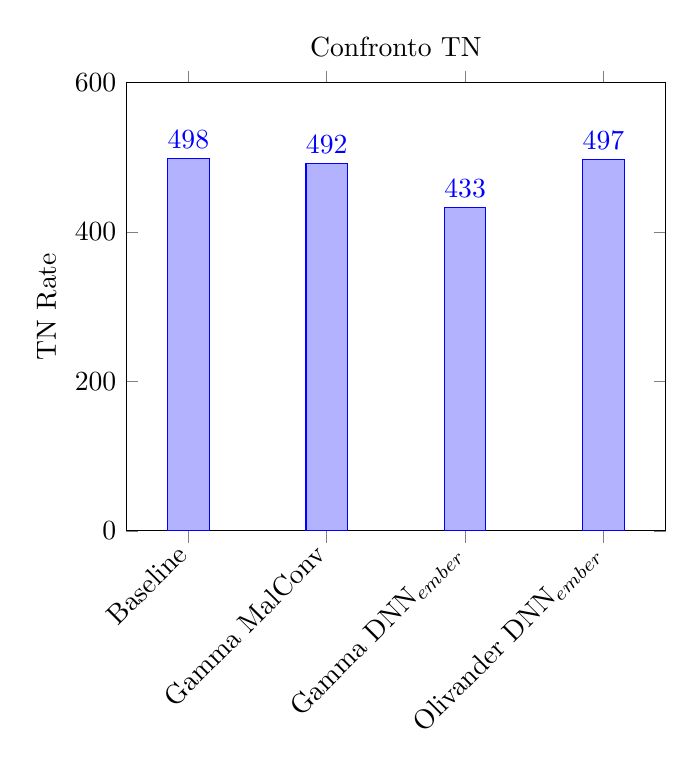
\begin{tikzpicture}
            \begin{axis}[
                ybar,
                symbolic x coords={Baseline, Gamma MalConv, Gamma DNN Ember, Olivander DNN Ember},
xticklabels={Baseline, Gamma MalConv, Gamma DNN$_{\text{ember}}$, Olivander DNN$_{\text{ember}}$},
                xticklabels={Baseline, Gamma MalConv, Gamma DNN$_{\text{ember}}$, Olivander DNN$_{\text{ember}}$},
                xtick=data,
                nodes near coords,
                ymin=0, ymax=600,
                ylabel={TN Rate},
                title={Confronto TN},
                x tick label style={rotate=45, anchor=east},
                bar width=15pt,
                enlarge x limits=0.15
            ]
                \addplot coordinates {(Baseline,498) (Gamma MalConv,492) (Gamma DNN Ember,433) (Olivander DNN Ember,497)};
            \end{axis}
        \end{tikzpicture}
        }
        \caption{Confronto TN}
        \label{fig:tn_comparison}
    \end{subfigure}
    \hfill
    \begin{subfigure}[b]{0.45\textwidth}
        \centering
        \resizebox{\textwidth}{!}{
        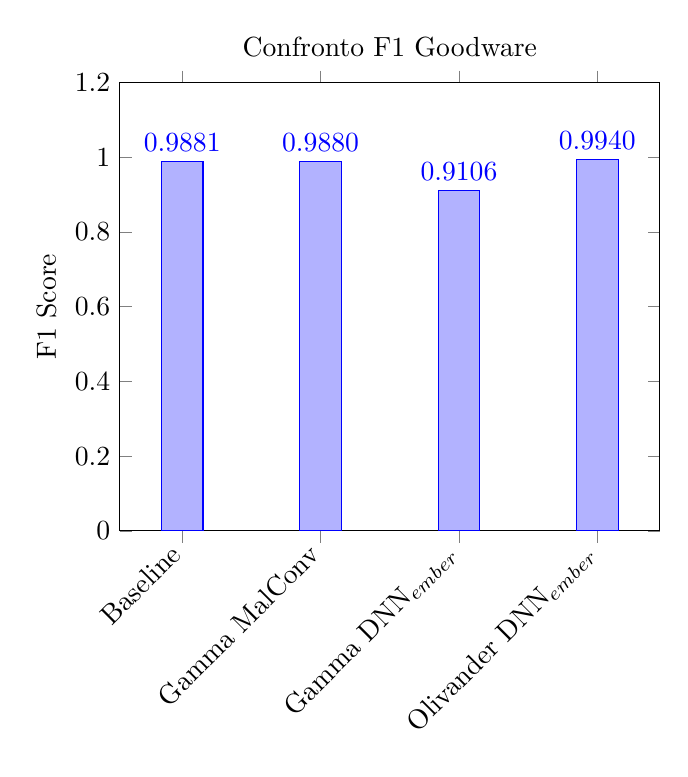
\begin{tikzpicture}
            \begin{axis}[
                ybar,
                symbolic x coords={Baseline, Gamma MalConv, Gamma DNN Ember, Olivander DNN Ember},
xticklabels={Baseline, Gamma MalConv, Gamma DNN$_{\text{ember}}$, Olivander DNN$_{\text{ember}}$},
                xtick=data,
                nodes near coords,
                nodes near coords style={/pgf/number format/.cd,fixed,precision=4,zerofill},
                ymin=0, ymax=1.2,
                ylabel={F1 Score},
                title={Confronto F1 Goodware},
                x tick label style={rotate=45, anchor=east},
                bar width=15pt,
                enlarge x limits=0.15
            ]
                \addplot coordinates {(Baseline,0.9881) (Gamma MalConv,0.9880) (Gamma DNN Ember,0.9106) (Olivander DNN Ember,0.9940)};
            \end{axis}
        \end{tikzpicture}
        }
        \caption{Confronto F1 Goodware}
        \label{fig:f1_goodware_comparison}
    \end{subfigure}
    
    \vspace{1cm}
    
    \begin{subfigure}[b]{0.45\textwidth}
        \centering
        \resizebox{\textwidth}{!}{
        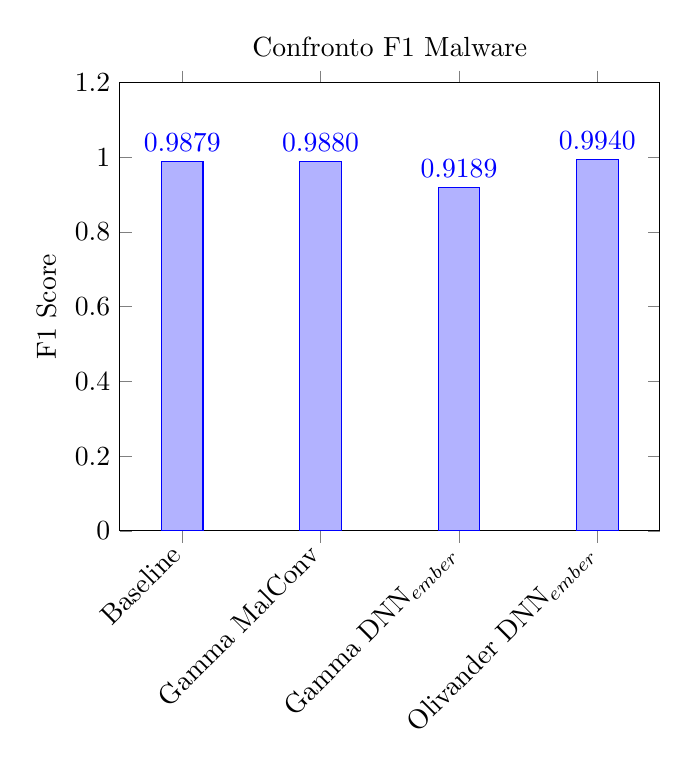
\begin{tikzpicture}
            \begin{axis}[
                ybar,
                symbolic x coords={Baseline, Gamma MalConv, Gamma DNN Ember, Olivander DNN Ember},
xticklabels={Baseline, Gamma MalConv, Gamma DNN$_{\text{ember}}$, Olivander DNN$_{\text{ember}}$},
xticklabels={Baseline, Gamma MalConv, Gamma DNN$_{\text{ember}}$, Olivander DNN$_{\text{ember}}$},
                xtick=data,
                nodes near coords,
                nodes near coords style={/pgf/number format/.cd,fixed,precision=4,zerofill},
                ymin=0, ymax=1.2,
                ylabel={F1 Score},
                title={Confronto F1 Malware},
                x tick label style={rotate=45, anchor=east},
                bar width=15pt,
                enlarge x limits=0.15
            ]
                \addplot coordinates {(Baseline,0.9879) (Gamma MalConv,0.9880) (Gamma DNN Ember,0.9189) (Olivander DNN Ember,0.9940)};
            \end{axis}
        \end{tikzpicture}
        }
        \caption{Confronto F1 Malware}
        \label{fig:f1_malware_comparison}
    \end{subfigure}
    \hfill
    \begin{subfigure}[b]{0.45\textwidth}
        \centering
        \resizebox{\textwidth}{!}{
        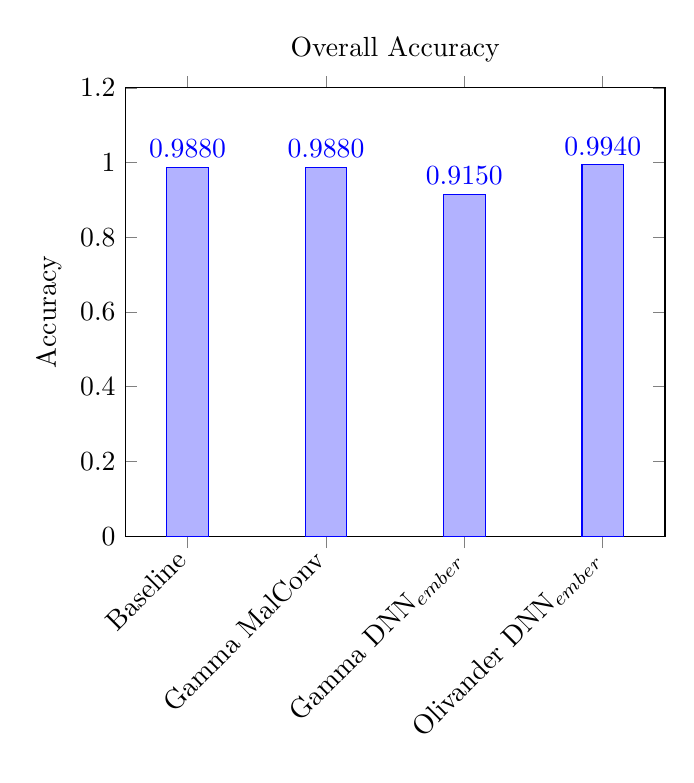
\begin{tikzpicture}
            \begin{axis}[
                ybar,
                symbolic x coords={Baseline, Gamma MalConv, Gamma DNN Ember, Olivander DNN Ember},
xticklabels={Baseline, Gamma MalConv, Gamma DNN$_{\text{ember}}$, Olivander DNN$_{\text{ember}}$},
xticklabels={Baseline, Gamma MalConv, Gamma DNN$_{\text{ember}}$, Olivander DNN$_{\text{ember}}$},
                xtick=data,
                nodes near coords,
                nodes near coords style={/pgf/number format/.cd,fixed,precision=4,zerofill},
                ymin=0, ymax=1.2,
                ylabel={Accuracy},
                title={Overall Accuracy},
                x tick label style={rotate=45, anchor=east},
                bar width=15pt,
                enlarge x limits=0.15
            ]
                \addplot coordinates {(Baseline,0.988) (Gamma MalConv,0.988) (Gamma DNN Ember,0.915) (Olivander DNN Ember,0.994)};
            \end{axis}
        \end{tikzpicture}
        }
        \caption{Overall Accuracy}
        \label{fig:accuracy_comparison}
    \end{subfigure}
    \caption{Confronto metriche - Label Flipping con Iniezione (unweighted)}
    \label{fig:poisoning_results}
\end{figure}

Poiché l'iniezione di campioni adversarial altera il bilanciamento del dataset, è stata condotta un'ulteriore analisi applicando un bilanciamento dei pesi delle classi (class weighting) durante l'addestramento, per compensare la nuova distribuzione. I risultati sono mostrati in Figura~\ref{fig:poisoning_results_weighted}.

L'applicazione del class weighting inverte significativamente i risultati osservati in precedenza. Come evidenziato dalla Figura~\ref{fig:poisoning_results_weighted}, l'attacco con GAMMA contro \(DNN_{ember}\), che senza pesatura risultava devastante, ora mostra un impatto contenuto (accuratezza 0.985 contro baseline 0.988). Viceversa, GAMMA contro MalConv e OLIVANDER contro \(DNN_{ember}\), precedentemente inefficaci, ora manifestano un degrado più pronunciato: l'accuratezza scende rispettivamente a 0.939 e 0.956, con una notevole riduzione dei TN. Questo comportamento suggerisce che il bilanciamento dei pesi costringe il modello a dare maggiore importanza ai campioni adversarial, amplificandone l'effetto distorsivo sul processo di apprendimento.

\begin{figure}[htbp]
    \centering
    \begin{subfigure}[b]{0.45\textwidth}
        \centering
        \resizebox{\textwidth}{!}{
        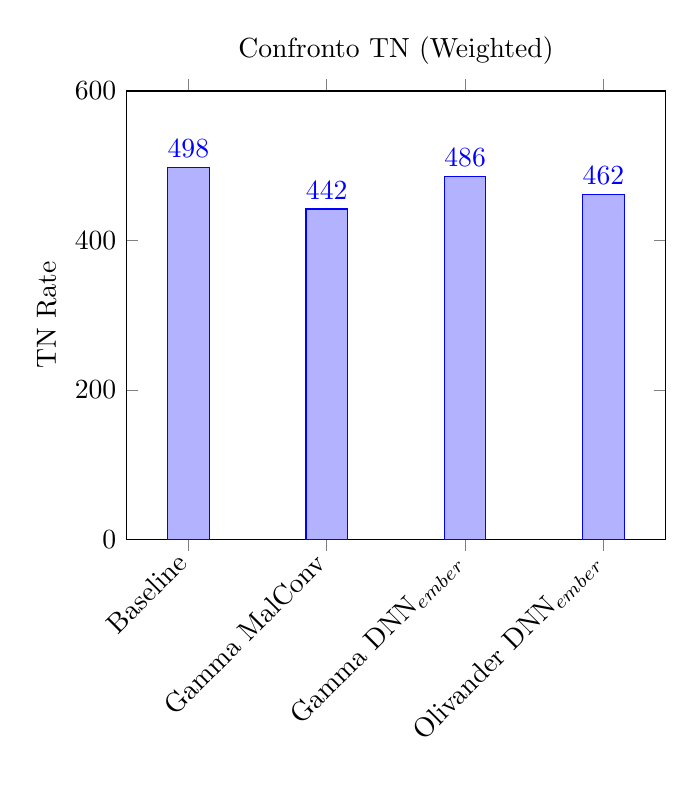
\begin{tikzpicture}
            \begin{axis}[
                ybar,
                symbolic x coords={Baseline, Gamma MalConv, Gamma DNN Ember, Olivander DNN Ember},
xticklabels={Baseline, Gamma MalConv, Gamma DNN$_{\text{ember}}$, Olivander DNN$_{\text{ember}}$},
                xtick=data,
                nodes near coords,
                ymin=0, ymax=600,
                ylabel={TN Rate},
                title={Confronto TN (Weighted)},
                x tick label style={rotate=45, anchor=east},
                bar width=15pt,
                enlarge x limits=0.15
            ]
                \addplot coordinates {(Baseline,498) (Gamma MalConv,442) (Gamma DNN Ember,486) (Olivander DNN Ember,462)};
            \end{axis}
        \end{tikzpicture}
        }
        \caption{Confronto TN}
        \label{fig:tn_comparison_weighted}
    \end{subfigure}
    \hfill
    \begin{subfigure}[b]{0.45\textwidth}
        \centering
        \resizebox{\textwidth}{!}{
        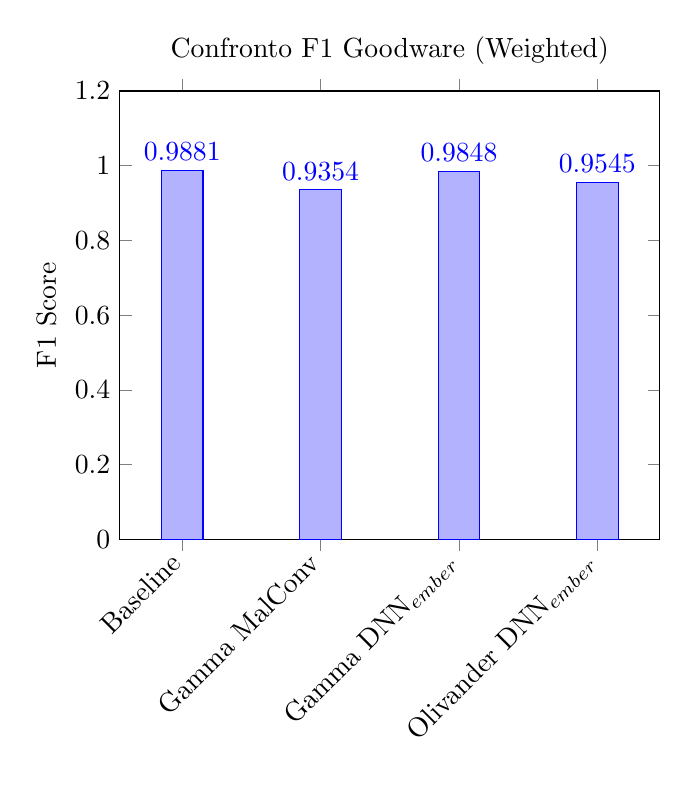
\begin{tikzpicture}
            \begin{axis}[
                ybar,
                symbolic x coords={Baseline, Gamma MalConv, Gamma DNN Ember, Olivander DNN Ember},
xticklabels={Baseline, Gamma MalConv, Gamma DNN$_{\text{ember}}$, Olivander DNN$_{\text{ember}}$},
                xtick=data,
                nodes near coords,
                nodes near coords style={/pgf/number format/.cd,fixed,precision=4,zerofill},
                ymin=0, ymax=1.2,
                ylabel={F1 Score},
                title={Confronto F1 Goodware (Weighted)},
                x tick label style={rotate=45, anchor=east},
                bar width=15pt,
                enlarge x limits=0.15
            ]
                \addplot coordinates {(Baseline,0.9881) (Gamma MalConv,0.9354) (Gamma DNN Ember,0.9848) (Olivander DNN Ember,0.9545)};
            \end{axis}
        \end{tikzpicture}
        }
        \caption{Confronto F1 Goodware}
        \label{fig:f1_goodware_comparison_weighted}
    \end{subfigure}
    
    \vspace{1cm}
    
    \begin{subfigure}[b]{0.45\textwidth}
        \centering
        \resizebox{\textwidth}{!}{
        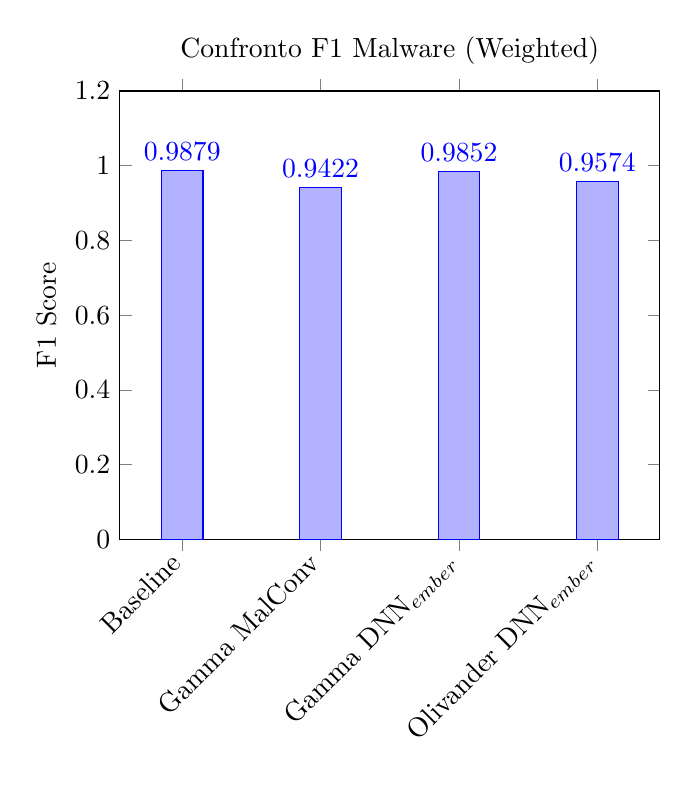
\begin{tikzpicture}
            \begin{axis}[
                ybar,
                symbolic x coords={Baseline, Gamma MalConv, Gamma DNN Ember, Olivander DNN Ember},
xticklabels={Baseline, Gamma MalConv, Gamma DNN$_{\text{ember}}$, Olivander DNN$_{\text{ember}}$},
                xtick=data,
                nodes near coords,
                nodes near coords style={/pgf/number format/.cd,fixed,precision=4,zerofill},
                ymin=0, ymax=1.2,
                ylabel={F1 Score},
                title={Confronto F1 Malware (Weighted)},
                x tick label style={rotate=45, anchor=east},
                bar width=15pt,
                enlarge x limits=0.15
            ]
                \addplot coordinates {(Baseline,0.987903226) (Gamma MalConv,0.942180095) (Gamma DNN Ember,0.985192498) (Olivander DNN Ember,0.957364341)};
            \end{axis}
        \end{tikzpicture}
        }
        \caption{Confronto F1 Malware}
        \label{fig:f1_malware_comparison_weighted}
    \end{subfigure}
    \hfill
    \begin{subfigure}[b]{0.45\textwidth}
        \centering
        \resizebox{\textwidth}{!}{
        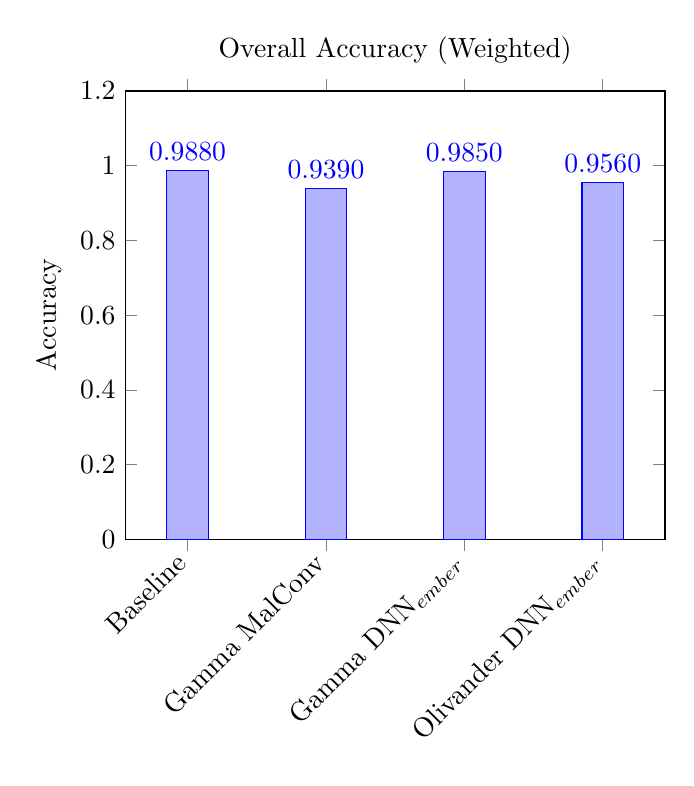
\begin{tikzpicture}
            \begin{axis}[
                ybar,
                symbolic x coords={Baseline, Gamma MalConv, Gamma DNN Ember, Olivander DNN Ember},
xticklabels={Baseline, Gamma MalConv, Gamma DNN$_{\text{ember}}$, Olivander DNN$_{\text{ember}}$},
                xtick=data,
                nodes near coords,
                nodes near coords style={/pgf/number format/.cd,fixed,precision=4,zerofill},
                ymin=0, ymax=1.2,
                ylabel={Accuracy},
                title={Overall Accuracy (Weighted)},
                x tick label style={rotate=45, anchor=east},
                bar width=15pt,
                enlarge x limits=0.15
            ]
                \addplot coordinates {(Baseline,0.988) (Gamma MalConv,0.939) (Gamma DNN Ember,0.985) (Olivander DNN Ember,0.956)};
            \end{axis}
        \end{tikzpicture}
        }
        \caption{Overall Accuracy}
        \label{fig:accuracy_comparison_weighted}
    \end{subfigure}
    \caption{Confronto metriche - Label Flipping con Iniezione (Weighted)}
    \label{fig:poisoning_results_weighted}
\end{figure}

Successivamente, l'analisi si è concentrata sulla variante dell'attacco tramite \textbf{label flipping con rimpiazzo}. In questo scenario, anziché aggiungere nuovi campioni, una porzione degli esempi originali del training set è stata sostituita con gli esempi adversarial, mantenendo l'etichetta invertita (Goodware). Tale approccio preserva la dimensione originale del dataset di addestramento. I grafici seguenti illustrano l'impatto di questa strategia sulle metriche di performance.

I risultati del label flipping con rimpiazzo, riportati in Figura~\ref{fig:poisoning_flipping_replacement}, mostrano un degrado prestazionale moderato ma uniforme per tutti gli attacchi considerati. L'accuratezza complessiva si attesta tra 0.949 e 0.960, con riduzioni dei TN comprese tra 30 e 46 unità rispetto alla baseline. Questo comportamento più omogeneo, rispetto alla variante con iniezione, è riconducibile al mantenimento del bilanciamento originale del dataset: sostituendo campioni della classe maggioritaria con esempi adversarial, il modello non è influenzato da sbilanciamenti artificiali e apprende in modo più stabile la distorsione introdotta. Tuttavia, l'impatto rimane significativo, evidenziando la vulnerabilità del processo di addestramento anche quando il dataset mantiene le proporzioni originali tra le classi, ed anche in questo caso GAMMA si dimostra piu efficace.

\begin{figure}[htbp]
    \centering
    \begin{subfigure}[b]{0.45\textwidth}
        \centering
        \resizebox{\textwidth}{!}{
        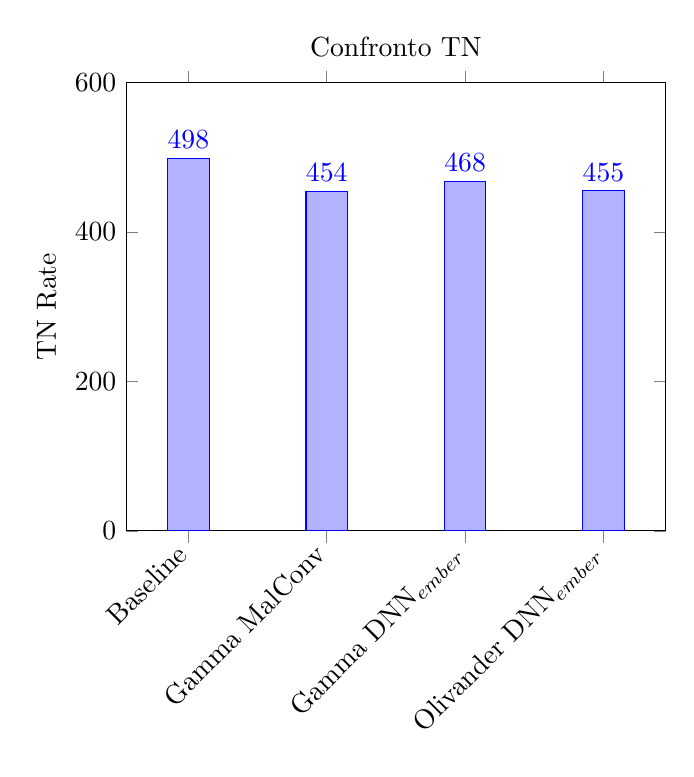
\begin{tikzpicture}
            \begin{axis}[
                ybar,
                symbolic x coords={Baseline, Gamma MalConv, Gamma DNN Ember, Olivander DNN Ember},
xticklabels={Baseline, Gamma MalConv, Gamma DNN$_{\text{ember}}$, Olivander DNN$_{\text{ember}}$},
                xtick=data,
                nodes near coords,
                ymin=0, ymax=600,
                ylabel={TN Rate},
                title={Confronto TN},
                x tick label style={rotate=45, anchor=east},
                bar width=15pt,
                enlarge x limits=0.15
            ]
                \addplot coordinates {(Baseline,498) (Gamma MalConv,454) (Gamma DNN Ember,468) (Olivander DNN Ember,455)};
            \end{axis}
        \end{tikzpicture}
        }
        \caption{Confronto TN}
        \label{fig:tn_comparison_flipping_replacement}
    \end{subfigure}
    \hfill
    \begin{subfigure}[b]{0.45\textwidth}
        \centering
        \resizebox{\textwidth}{!}{
        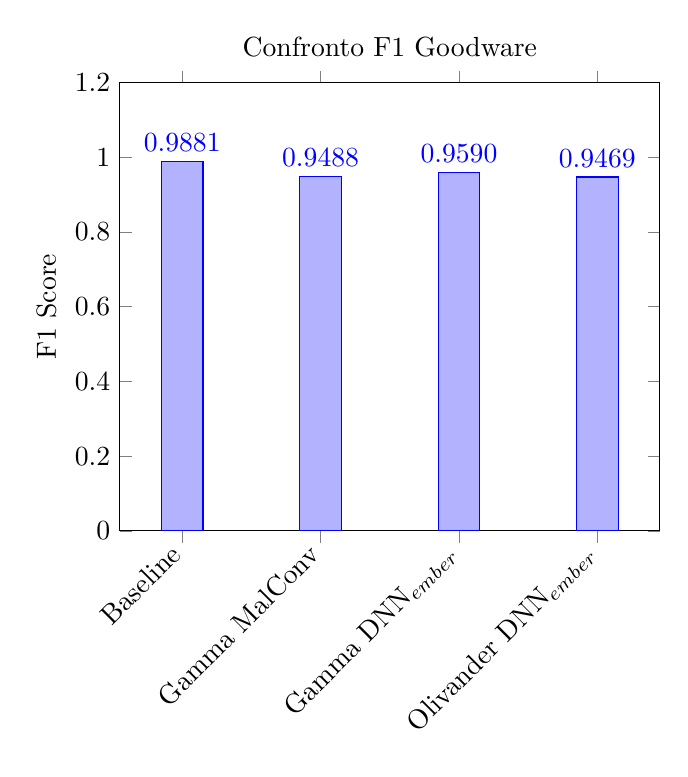
\begin{tikzpicture}
            \begin{axis}[
                ybar,
                symbolic x coords={Baseline, Gamma MalConv, Gamma DNN Ember, Olivander DNN Ember},
xticklabels={Baseline, Gamma MalConv, Gamma DNN$_{\text{ember}}$, Olivander DNN$_{\text{ember}}$},
                xtick=data,
                nodes near coords,
                nodes near coords style={/pgf/number format/.cd,fixed,precision=4,zerofill},
                ymin=0, ymax=1.2,
                ylabel={F1 Score},
                title={Confronto F1 Goodware},
                x tick label style={rotate=45, anchor=east},
                bar width=15pt,
                enlarge x limits=0.15
            ]
                \addplot coordinates {(Baseline,0.9881) (Gamma MalConv,0.9488) (Gamma DNN Ember,0.959) (Olivander DNN Ember,0.9469)};
            \end{axis}
        \end{tikzpicture}
        }
        \caption{Confronto F1 Goodware}
        \label{fig:f1_goodware_comparison_flipping_replacement}
    \end{subfigure}
    
    \vspace{1cm}
    
    \begin{subfigure}[b]{0.45\textwidth}
        \centering
        \resizebox{\textwidth}{!}{
        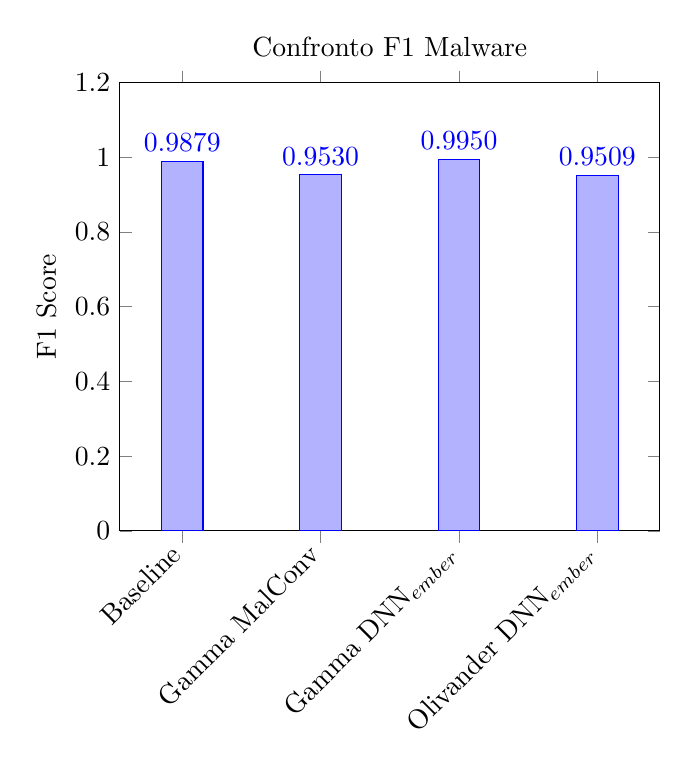
\begin{tikzpicture}
            \begin{axis}[
                ybar,
                symbolic x coords={Baseline, Gamma MalConv, Gamma DNN Ember, Olivander DNN Ember},
xticklabels={Baseline, Gamma MalConv, Gamma DNN$_{\text{ember}}$, Olivander DNN$_{\text{ember}}$},
                xtick=data,
                nodes near coords,
                nodes near coords style={/pgf/number format/.cd,fixed,precision=4,zerofill},
                ymin=0, ymax=1.2,
                ylabel={F1 Score},
                title={Confronto F1 Malware},
                x tick label style={rotate=45, anchor=east},
                bar width=15pt,
                enlarge x limits=0.15
            ]
                \addplot coordinates {(Baseline,0.9879) (Gamma MalConv,0.9530) (Gamma DNN Ember,0.9950) (Olivander DNN Ember,0.9509)};
            \end{axis}
        \end{tikzpicture}
        }
        \caption{Confronto F1 Malware}
        \label{fig:f1_malware_comparison_flipping_replacement}
    \end{subfigure}
    \hfill
    \begin{subfigure}[b]{0.45\textwidth}
        \centering
        \resizebox{\textwidth}{!}{
        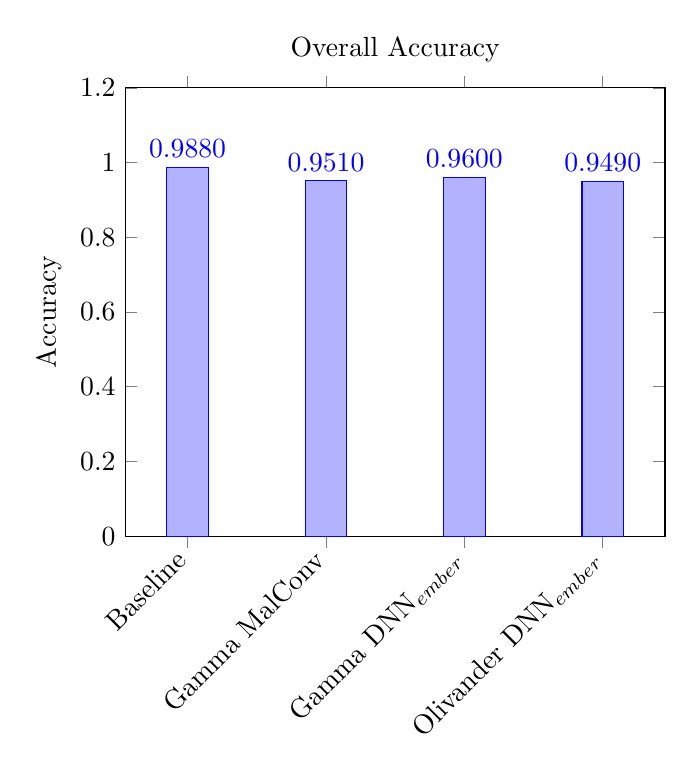
\begin{tikzpicture}
            \begin{axis}[
                ybar,
                symbolic x coords={Baseline, Gamma MalConv, Gamma DNN Ember, Olivander DNN Ember},
xticklabels={Baseline, Gamma MalConv, Gamma DNN$_{\text{ember}}$, Olivander DNN$_{\text{ember}}$},
                xtick=data,
                nodes near coords,
                nodes near coords style={/pgf/number format/.cd,fixed,precision=4,zerofill},
                ymin=0, ymax=1.2,
                ylabel={Accuracy},
                title={Overall Accuracy},
                x tick label style={rotate=45, anchor=east},
                bar width=15pt,
                enlarge x limits=0.15
            ]
                \addplot coordinates {(Baseline,0.988) (Gamma MalConv,0.951) (Gamma DNN Ember,0.960) (Olivander DNN Ember,0.949)};
            \end{axis}
        \end{tikzpicture}
        }
        \caption{Overall Accuracy}
        \label{fig:accuracy_comparison_flipping_replacement}
    \end{subfigure}
    \caption{Confronto metriche - Label Flipping con Rimpiazzo}
    \label{fig:poisoning_flipping_replacement}
\end{figure}

La sezione seguente espone i risultati relativi all'attacco \textbf{clean label con iniezione}. A differenza del label flipping, in questa configurazione gli esempi adversarial vengono aggiunti al training set mantenendo la loro etichetta corretta (Malware). Le figure sottostanti mostrano il confronto con la baseline.

Come evidenziato dalla Figura~\ref{fig:poisoning_clean_injection}, l'attacco clean label con iniezione risulta completamente inefficace: non solo non degrada le performance del modello target, ma in alcuni casi le migliora leggermente, con accuratezze fino a 0.998 per OLIVANDER e 0.997 per GAMMA contro \(DNN_{ember}\). Questo risultato non è affatto sorprendente se si considera che la procedura di clean label poisoning è sostanzialmente identica all'adversarial training, una tecnica consolidata per migliorare la robustezza dei modelli. L'aggiunta di esempi malware perturbati con la loro etichetta corretta funziona come una forma di data augmentation, arricchendo il training set con campioni difficili che aiutano il modello a generalizzare meglio.

L'inefficacia di questa strategia dimostra che né GAMMA né OLIVANDER sono stati progettati per realizzare la feature collision descritta nel capitolo precedente. Se gli attacchi mirassero a far collassare le rappresentazioni di malware e goodware nello spazio delle feature, l'aggiunta di esempi con etichetta corretta dovrebbe comunque confondere il confine decisionale. Al contrario, i risultati indicano che gli esempi adversarial generati, pur essendo efficaci in fase di evasion, mantengono caratteristiche sufficientemente distintive da essere correttamente appresi quando etichettati come malware. Studi recenti~\cite{Lobascio2025Adversarial} hanno infatti utilizzato GAMMA per la creazione di esempi adversarial per scopi di adversarial training.

\begin{figure}[htbp]
    \centering
    \begin{subfigure}[b]{0.45\textwidth}
        \centering
        \resizebox{\textwidth}{!}{
        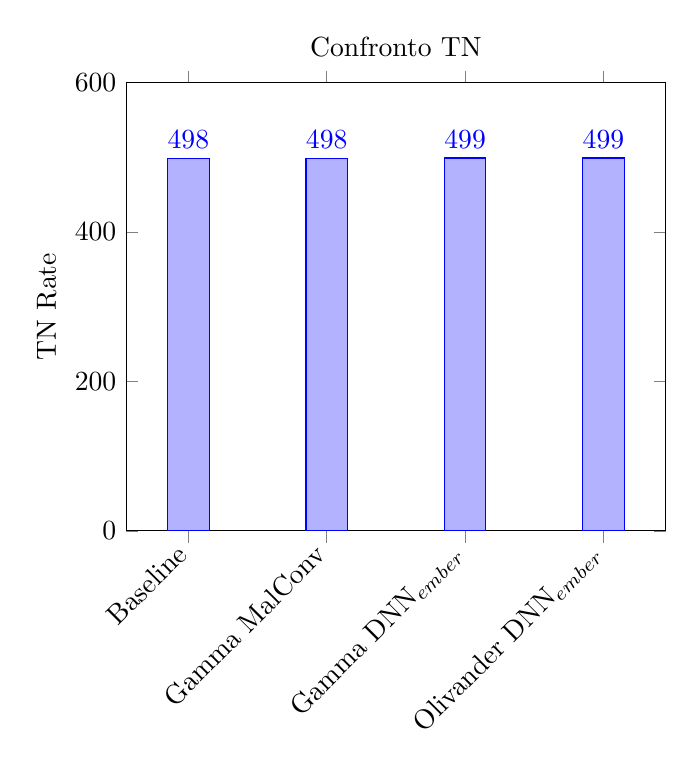
\begin{tikzpicture}
            \begin{axis}[
                ybar,
                symbolic x coords={Baseline, Gamma MalConv, Gamma DNN Ember, Olivander DNN Ember},
xticklabels={Baseline, Gamma MalConv, Gamma DNN$_{\text{ember}}$, Olivander DNN$_{\text{ember}}$},
                xtick=data,
                nodes near coords,
                ymin=0, ymax=600,
                ylabel={TN Rate},
                title={Confronto TN},
                x tick label style={rotate=45, anchor=east},
                bar width=15pt,
                enlarge x limits=0.15
            ]
                \addplot coordinates {(Baseline,498) (Gamma MalConv,498) (Gamma DNN Ember,499) (Olivander DNN Ember,499)};
            \end{axis}
        \end{tikzpicture}
        }
        \caption{Confronto TN}
        \label{fig:tn_comparison_clean_injection}
    \end{subfigure}
    \hfill
    \begin{subfigure}[b]{0.45\textwidth}
        \centering
        \resizebox{\textwidth}{!}{
        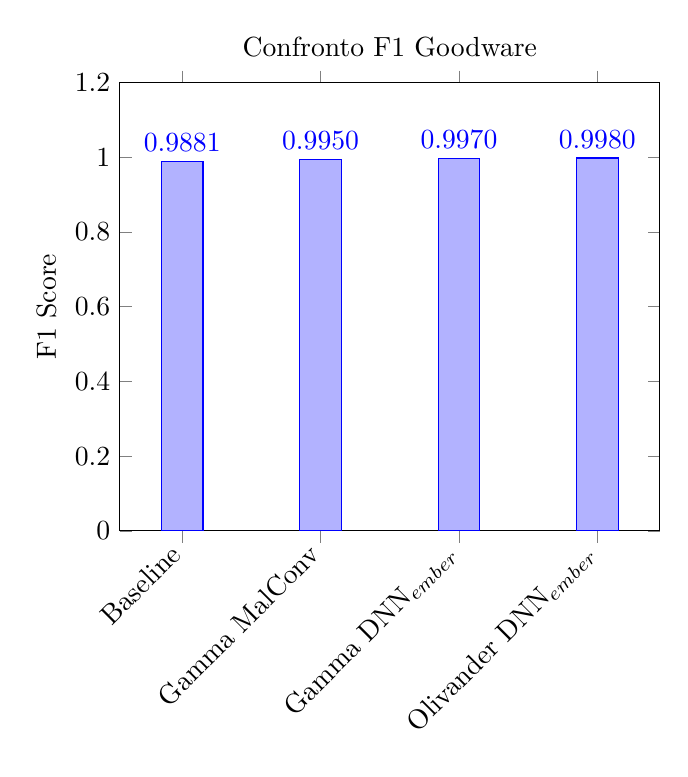
\begin{tikzpicture}
            \begin{axis}[
                ybar,
                symbolic x coords={Baseline, Gamma MalConv, Gamma DNN Ember, Olivander DNN Ember},
xticklabels={Baseline, Gamma MalConv, Gamma DNN$_{\text{ember}}$, Olivander DNN$_{\text{ember}}$},
                xtick=data,
                nodes near coords,
                nodes near coords style={/pgf/number format/.cd,fixed,precision=4,zerofill},
                ymin=0, ymax=1.2,
                ylabel={F1 Score},
                title={Confronto F1 Goodware},
                x tick label style={rotate=45, anchor=east},
                bar width=15pt,
                enlarge x limits=0.15
            ]
                \addplot coordinates {(Baseline,0.9881) (Gamma MalConv,0.9950) (Gamma DNN Ember,0.9970) (Olivander DNN Ember,0.9980)};
            \end{axis}
        \end{tikzpicture}
        }
        \caption{Confronto F1 Goodware}
        \label{fig:f1_goodware_comparison_clean_injection}
    \end{subfigure}
    
    \vspace{1cm}
    
    \begin{subfigure}[b]{0.45\textwidth}
        \centering
        \resizebox{\textwidth}{!}{
        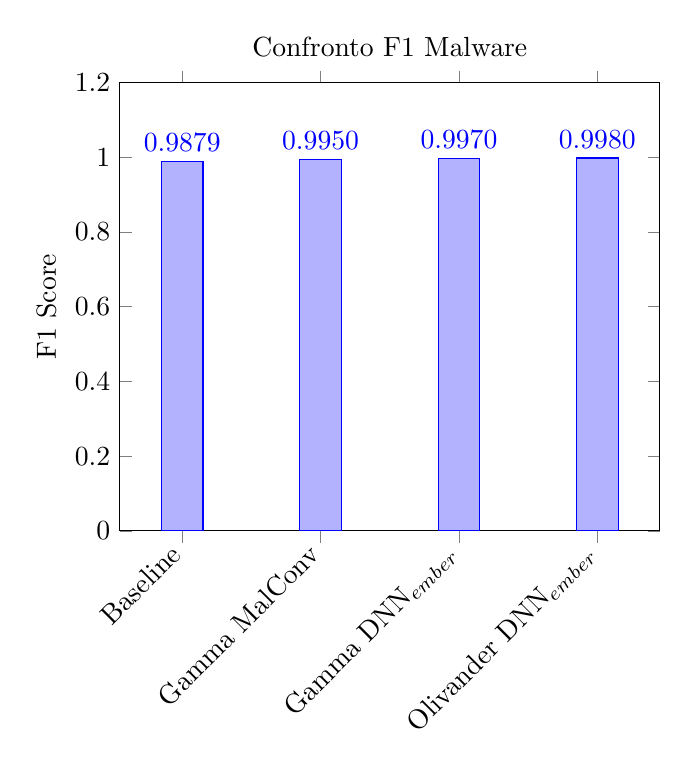
\begin{tikzpicture}
            \begin{axis}[
                ybar,
                symbolic x coords={Baseline, Gamma MalConv, Gamma DNN Ember, Olivander DNN Ember},
xticklabels={Baseline, Gamma MalConv, Gamma DNN$_{\text{ember}}$, Olivander DNN$_{\text{ember}}$},
                xtick=data,
                nodes near coords,
                nodes near coords style={/pgf/number format/.cd,fixed,precision=4,zerofill},
                ymin=0, ymax=1.2,
                ylabel={F1 Score},
                title={Confronto F1 Malware},
                x tick label style={rotate=45, anchor=east},
                bar width=15pt,
                enlarge x limits=0.15
            ]
                \addplot coordinates {(Baseline,0.9879) (Gamma MalConv,0.9950) (Gamma DNN Ember,0.997002997) (Olivander DNN Ember,0.998)};
            \end{axis}
        \end{tikzpicture}
        }
        \caption{Confronto F1 Malware}
        \label{fig:f1_malware_comparison_clean_injection}
    \end{subfigure}
    \hfill
    \begin{subfigure}[b]{0.45\textwidth}
        \centering
        \resizebox{\textwidth}{!}{
        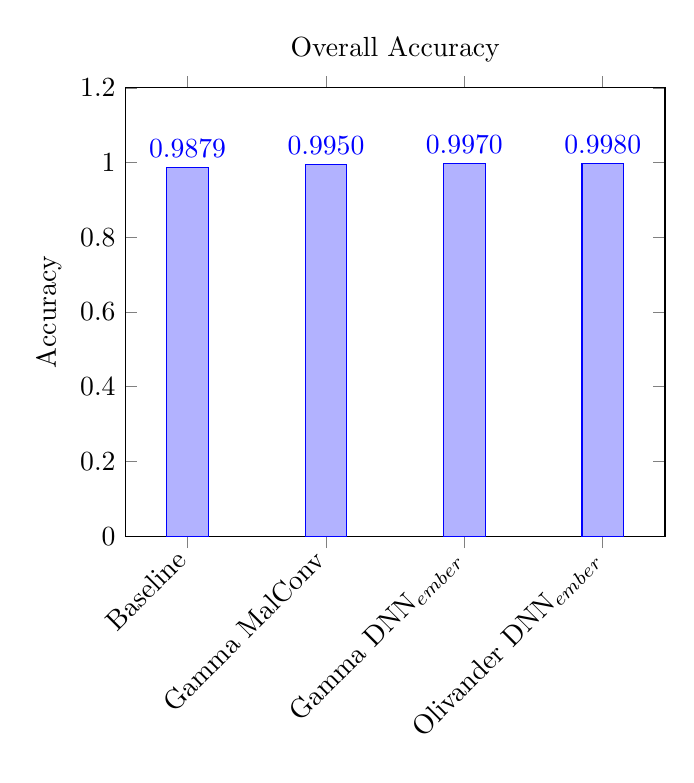
\begin{tikzpicture}
            \begin{axis}[
                ybar,
                symbolic x coords={Baseline, Gamma MalConv, Gamma DNN Ember, Olivander DNN Ember},
xticklabels={Baseline, Gamma MalConv, Gamma DNN$_{\text{ember}}$, Olivander DNN$_{\text{ember}}$},
                xtick=data,
                nodes near coords,
                nodes near coords style={/pgf/number format/.cd,fixed,precision=4,zerofill},
                ymin=0, ymax=1.2,
                ylabel={Accuracy},
                title={Overall Accuracy},
                x tick label style={rotate=45, anchor=east},
                bar width=15pt,
                enlarge x limits=0.15
            ]
                \addplot coordinates {(Baseline,0.9879) (Gamma MalConv,0.994994995) (Gamma DNN Ember,0.997002997) (Olivander DNN Ember,0.998)};
            \end{axis}
        \end{tikzpicture}
        }
        \caption{Overall Accuracy}
        \label{fig:accuracy_comparison_clean_injection}
    \end{subfigure}
    \caption{Confronto metriche - Clean Label con Iniezione}
    \label{fig:poisoning_clean_injection}
\end{figure}

Analogamente a quanto fatto per il label flipping, anche nel caso dell'attacco clean label con iniezione è stato valutato l'effetto del bilanciamento dei pesi delle classi, per mitigare lo sbilanciamento introdotto dall'aggiunta degli esempi adversarial. I grafici seguenti riportano i risultati ottenuti.

Come evidenziato dalla Figura~\ref{fig:poisoning_clean_injection_weighted}, l'applicazione del class weighting non altera sostanzialmente i risultati ottenuti senza pesatura. Le performance rimangono elevate, con accuratezze comprese tra 0.995 e 0.998, confermando che l'attacco clean label con iniezione è inefficace indipendentemente dalla strategia di bilanciamento adottata. Questo ulteriormente consolida la conclusione che GAMMA e OLIVANDER non sono ottimizzati per la feature collision: quando gli esempi adversarial sono correttamente etichettati, essi fungono da campioni di addestramento supplementari che, pur essendo difficili, contribuiscono positivamente all'apprendimento del modello anziché comprometterlo.

\begin{figure}[htbp]
    \centering
    \begin{subfigure}[b]{0.45\textwidth}
        \centering
        \resizebox{\textwidth}{!}{
        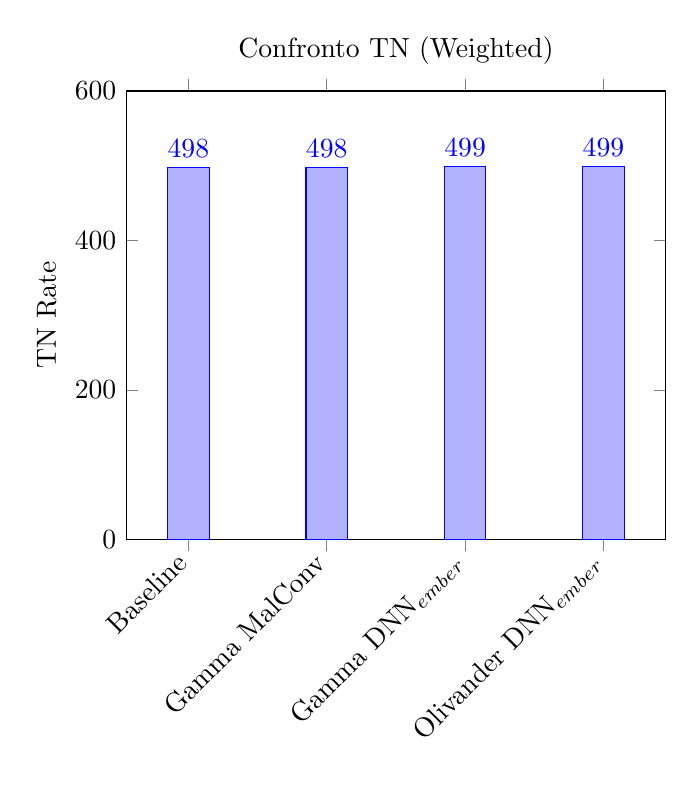
\begin{tikzpicture}
            \begin{axis}[
                ybar,
                symbolic x coords={Baseline, Gamma MalConv, Gamma DNN Ember, Olivander DNN Ember},
xticklabels={Baseline, Gamma MalConv, Gamma DNN$_{\text{ember}}$, Olivander DNN$_{\text{ember}}$},
                xtick=data,
                nodes near coords,
                ymin=0, ymax=600,
                ylabel={TN Rate},
                title={Confronto TN (Weighted)},
                x tick label style={rotate=45, anchor=east},
                bar width=15pt,
                enlarge x limits=0.15
            ]
                \addplot coordinates {(Baseline,498) (Gamma MalConv,498) (Gamma DNN Ember,499) (Olivander DNN Ember,499)};
            \end{axis}
        \end{tikzpicture}
        }
        \caption{Confronto TN}
        \label{fig:tn_comparison_clean_injection_weighted}
    \end{subfigure}
    \hfill
    \begin{subfigure}[b]{0.45\textwidth}
        \centering
        \resizebox{\textwidth}{!}{
        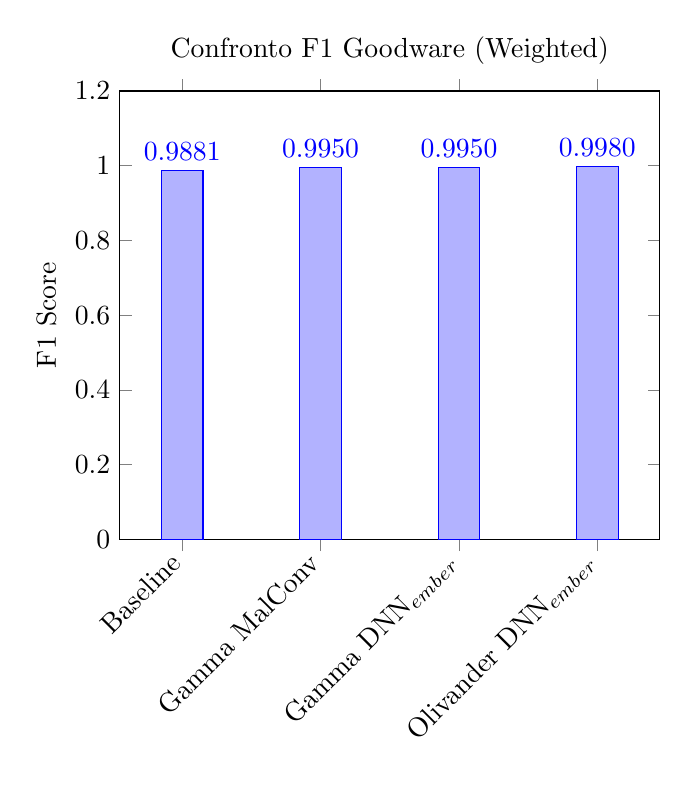
\begin{tikzpicture}
            \begin{axis}[
                ybar,
                symbolic x coords={Baseline, Gamma MalConv, Gamma DNN Ember, Olivander DNN Ember},
xticklabels={Baseline, Gamma MalConv, Gamma DNN$_{\text{ember}}$, Olivander DNN$_{\text{ember}}$},
                xtick=data,
                nodes near coords,
                nodes near coords style={/pgf/number format/.cd,fixed,precision=4,zerofill},
                ymin=0, ymax=1.2,
                ylabel={F1 Score},
                title={Confronto F1 Goodware (Weighted)},
                x tick label style={rotate=45, anchor=east},
                bar width=15pt,
                enlarge x limits=0.15
            ]
                \addplot coordinates {(Baseline,0.9881) (Gamma MalConv,0.9950) (Gamma DNN Ember,0.9950) (Olivander DNN Ember,0.9980)};
            \end{axis}
        \end{tikzpicture}
        }
        \caption{Confronto F1 Goodware}
        \label{fig:f1_goodware_comparison_clean_injection_weighted}
    \end{subfigure}
    
    \vspace{1cm}
    
    \begin{subfigure}[b]{0.45\textwidth}
        \centering
        \resizebox{\textwidth}{!}{
        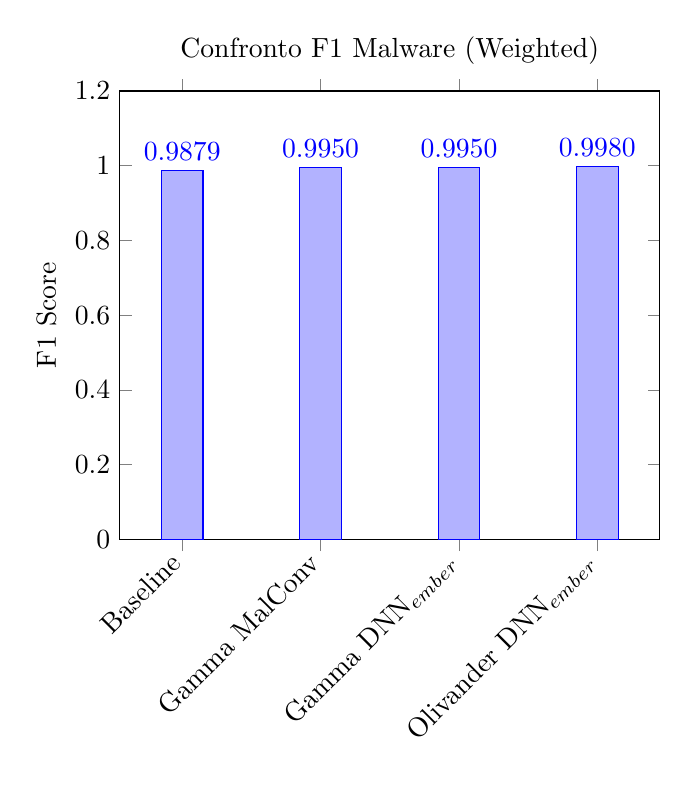
\begin{tikzpicture}
            \begin{axis}[
                ybar,
                symbolic x coords={Baseline, Gamma MalConv, Gamma DNN Ember, Olivander DNN Ember},
xticklabels={Baseline, Gamma MalConv, Gamma DNN$_{\text{ember}}$, Olivander DNN$_{\text{ember}}$},
                xtick=data,
                nodes near coords,
                nodes near coords style={/pgf/number format/.cd,fixed,precision=4,zerofill},
                ymin=0, ymax=1.2,
                ylabel={F1 Score},
                title={Confronto F1 Malware (Weighted)},
                x tick label style={rotate=45, anchor=east},
                bar width=15pt,
                enlarge x limits=0.15
            ]
                \addplot coordinates {(Baseline,0.987903226) (Gamma MalConv,0.994994995) (Gamma DNN Ember,0.994994995) (Olivander DNN Ember,0.998)};
            \end{axis}
        \end{tikzpicture}
        }
        \caption{Confronto F1 Malware}
        \label{fig:f1_malware_comparison_clean_injection_weighted}
    \end{subfigure}
    \hfill
    \begin{subfigure}[b]{0.45\textwidth}
        \centering
        \resizebox{\textwidth}{!}{
        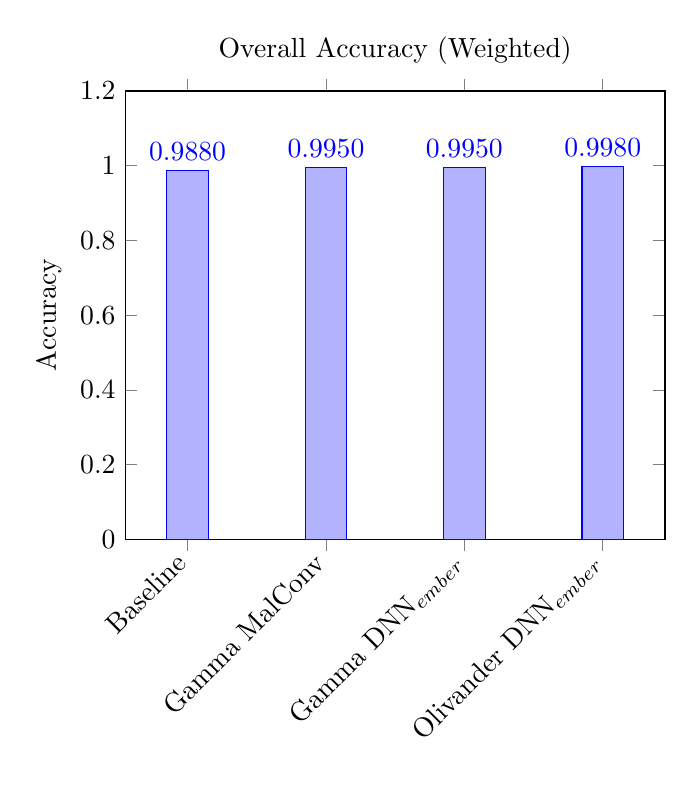
\begin{tikzpicture}
            \begin{axis}[
                ybar,
                symbolic x coords={Baseline, Gamma MalConv, Gamma DNN Ember, Olivander DNN Ember},
xticklabels={Baseline, Gamma MalConv, Gamma DNN$_{\text{ember}}$, Olivander DNN$_{\text{ember}}$},
                xtick=data,
                nodes near coords,
                nodes near coords style={/pgf/number format/.cd,fixed,precision=4,zerofill},
                ymin=0, ymax=1.2,
                ylabel={Accuracy},
                title={Overall Accuracy (Weighted)},
                x tick label style={rotate=45, anchor=east},
                bar width=15pt,
                enlarge x limits=0.15
            ]
                \addplot coordinates {(Baseline,0.988) (Gamma MalConv,0.9950) (Gamma DNN Ember,0.9950) (Olivander DNN Ember,0.9980)};
            \end{axis}
        \end{tikzpicture}
        }
        \caption{Overall Accuracy}
        \label{fig:accuracy_comparison_clean_injection_weighted}
    \end{subfigure}
    \caption{Confronto metriche - Clean Label con Iniezione (Weighted)}
    \label{fig:poisoning_clean_injection_weighted}
\end{figure}

Infine, è stato valutato l'impatto dell'attacco \textbf{clean label con rimpiazzo}. Analogamente al caso precedente, gli esempi adversarial vengono introdotti con la loro etichetta reale (Goodware), ma sostituiscono i campioni originali corrispondenti nel training set. Questa tecnica permette di isolare l'effetto della sostituzione di campioni ``puliti'' con campioni ``avversari'' sulla robustezza del modello, a parità di cardinalità del dataset. I risultati sono riportati nei grafici seguenti.

La Figura~\ref{fig:poisoning_clean_replacement} rivela un comportamento intermedio rispetto alle configurazioni precedenti. A differenza dell'iniezione, che migliorava le performance, il rimpiazzo determina un degrado misurabile ma contenuto: l'accuratezza si riduce a 0.976 per GAMMA contro MalConv e 0.977 per OLIVANDER contro \(DNN_{ember}\), con riduzioni dei TN rispettivamente di 23 e 20 unità. L'attacco con GAMMA contro \(DNN_{ember}\) rimane invece sostanzialmente inefficace. Questo degrado limitato è attribuibile alla riduzione della diversità del training set: sostituendo campioni goodware originali con versioni adversarial, si diminuisce la variabilità degli esempi disponibili per l'apprendimento, limitando la capacità del modello di generalizzare. Tuttavia, l'impatto rimane modesto, confermando nuovamente che l'etichettatura corretta neutralizza l'effetto distorsivo degli esempi adversarial.

\begin{figure}[htbp]
    \centering
    \begin{subfigure}[b]{0.45\textwidth}
        \centering
        \resizebox{\textwidth}{!}{
        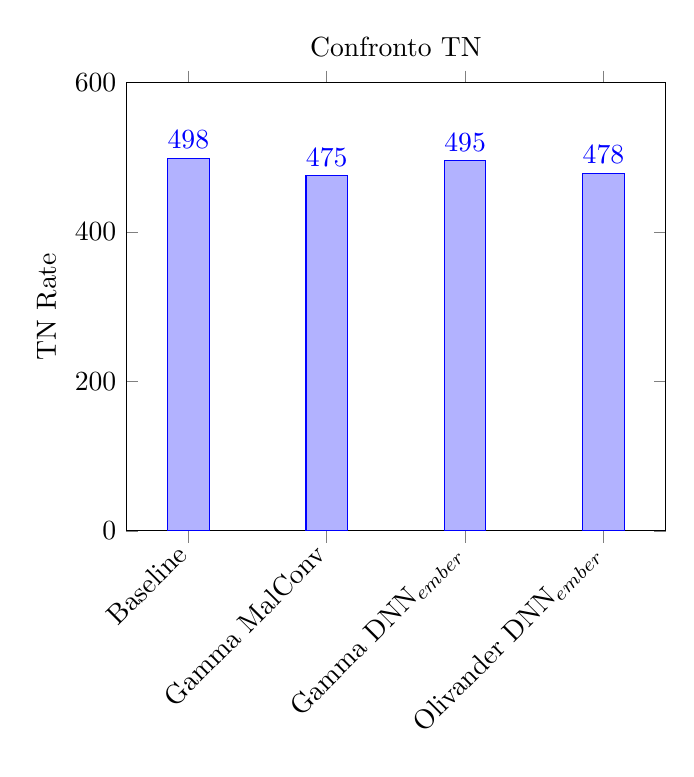
\begin{tikzpicture}
            \begin{axis}[
                ybar,
                symbolic x coords={Baseline, Gamma MalConv, Gamma DNN Ember, Olivander DNN Ember},
xticklabels={Baseline, Gamma MalConv, Gamma DNN$_{\text{ember}}$, Olivander DNN$_{\text{ember}}$},
                xtick=data,
                nodes near coords,
                ymin=0, ymax=600,
                ylabel={TN Rate},
                title={Confronto TN},
                x tick label style={rotate=45, anchor=east},
                bar width=15pt,
                enlarge x limits=0.15
            ]
                \addplot coordinates {(Baseline,498) (Gamma MalConv,475) (Gamma DNN Ember,495) (Olivander DNN Ember,478)};
            \end{axis}
        \end{tikzpicture}
        }
        \caption{Confronto TN}
        \label{fig:tn_comparison_clean_replacement}
    \end{subfigure}
    \hfill
    \begin{subfigure}[b]{0.45\textwidth}
        \centering
        \resizebox{\textwidth}{!}{
        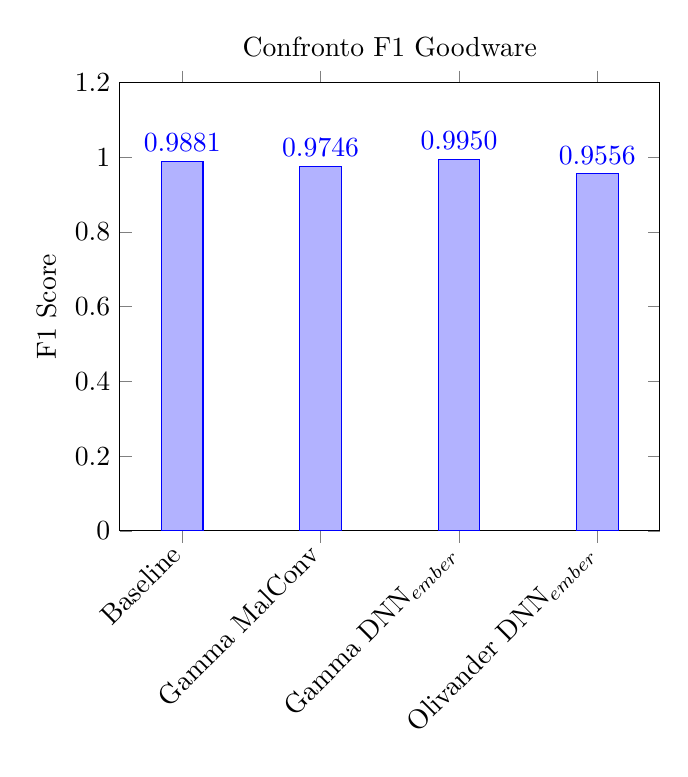
\begin{tikzpicture}
            \begin{axis}[
                ybar,
                symbolic x coords={Baseline, Gamma MalConv, Gamma DNN Ember, Olivander DNN Ember},
xticklabels={Baseline, Gamma MalConv, Gamma DNN$_{\text{ember}}$, Olivander DNN$_{\text{ember}}$},
                xtick=data,
                nodes near coords,
                nodes near coords style={/pgf/number format/.cd,fixed,precision=4,zerofill},
                ymin=0, ymax=1.2,
                ylabel={F1 Score},
                title={Confronto F1 Goodware},
                x tick label style={rotate=45, anchor=east},
                bar width=15pt,
                enlarge x limits=0.15
            ]
                \addplot coordinates {(Baseline,0.9881) (Gamma MalConv,0.9746) (Gamma DNN Ember,0.9950) (Olivander DNN Ember,0.9556)};
            \end{axis}
        \end{tikzpicture}
        }
        \caption{Confronto F1 Goodware}
        \label{fig:f1_goodware_comparison_clean_replacement}
    \end{subfigure}
    
    \vspace{1cm}
    
    \begin{subfigure}[b]{0.45\textwidth}
        \centering
        \resizebox{\textwidth}{!}{
        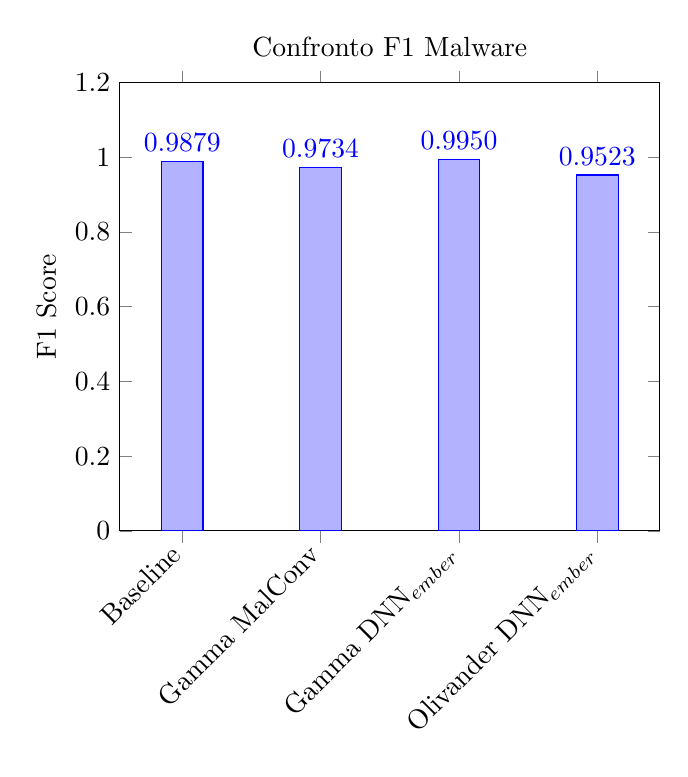
\begin{tikzpicture}
            \begin{axis}[
                ybar,
                symbolic x coords={Baseline, Gamma MalConv, Gamma DNN Ember, Olivander DNN Ember},
xticklabels={Baseline, Gamma MalConv, Gamma DNN$_{\text{ember}}$, Olivander DNN$_{\text{ember}}$},
                xtick=data,
                nodes near coords,
                nodes near coords style={/pgf/number format/.cd,fixed,precision=4,zerofill},
                ymin=0, ymax=1.2,
                ylabel={F1 Score},
                title={Confronto F1 Malware},
                x tick label style={rotate=45, anchor=east},
                bar width=15pt,
                enlarge x limits=0.15
            ]
                \addplot coordinates {(Baseline,0.9879) (Gamma MalConv,0.9734) (Gamma DNN Ember,0.9950) (Olivander DNN Ember,0.9523)};
            \end{axis}
        \end{tikzpicture}
        }
        \caption{Confronto F1 Malware}
        \label{fig:f1_malware_comparison_clean_replacement}
    \end{subfigure}
    \hfill
    \begin{subfigure}[b]{0.45\textwidth}
        \centering
        \resizebox{\textwidth}{!}{
        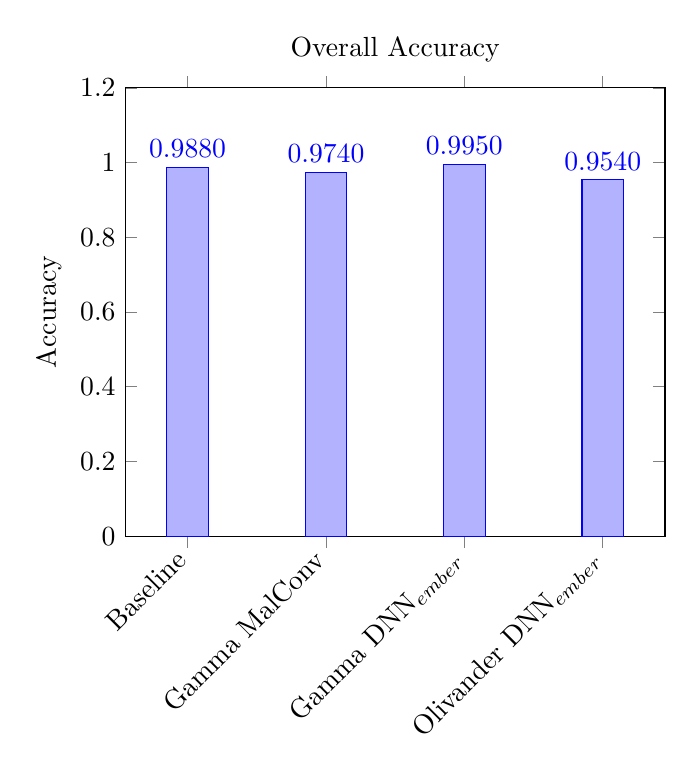
\begin{tikzpicture}
            \begin{axis}[
                ybar,
                symbolic x coords={Baseline, Gamma MalConv, Gamma DNN Ember, Olivander DNN Ember},
xticklabels={Baseline, Gamma MalConv, Gamma DNN$_{\text{ember}}$, Olivander DNN$_{\text{ember}}$},
                xtick=data,
                nodes near coords,
                nodes near coords style={/pgf/number format/.cd,fixed,precision=4,zerofill},
                ymin=0, ymax=1.2,
                ylabel={Accuracy},
                title={Overall Accuracy},
                x tick label style={rotate=45, anchor=east},
                bar width=15pt,
                enlarge x limits=0.15
            ]
                \addplot coordinates {(Baseline,0.988) (Gamma MalConv,0.974) (Gamma DNN Ember,0.995) (Olivander DNN Ember,0.954)};
            \end{axis}
        \end{tikzpicture}
        }
        \caption{Overall Accuracy}
        \label{fig:accuracy_comparison_clean_replacement}
    \end{subfigure}
    \caption{Confronto metriche - Clean Label con Rimpiazzo}
    \label{fig:poisoning_clean_replacement}
\end{figure}

A conclusione dell'analisi sperimentale, è stato condotto un ulteriore esperimento focalizzato sull'attacco OLIVANDER, confrontando l'efficacia dell'attacco standard con una variante in cui vengono iniettati solo i campioni adversarial rilevati come malware anche da VirusTotal (VT Filtered).
Questo confronto è stato eseguito sia per la strategia di \textit{Label Flipping} che per quella \textit{Clean Label}. Inoltre, per entrambe le configurazioni, è stato valutato l'impatto del bilanciamento dei pesi delle classi (\textit{Weighted}) per compensare lo sbilanciamento introdotto dall'iniezione.
La Figura \ref{fig:poisoning_olivander_vt_comparison} mostra i risultati senza bilanciamento, mentre la Figura \ref{fig:poisoning_olivander_vt_comparison_weighted} illustra i risultati ottenuti applicando il class weighting.

\begin{table}[htbp]
    \centering
    \caption{Numero di esempi adversarial utilizzati nel poisoning: Standard vs VT Filtered}
    \label{tab:vt_filtered_count}
    \begin{tabular}{lcc}
        \toprule
        \textbf{Strategia} & \textbf{Esempi Totali} & \textbf{Esempi VT Filtered} \\
        \midrule
        OLIVANDER & 1435 & 652 \\ % TODO: Inserire il numero corretto di esempi VT Filtered
        \bottomrule
    \end{tabular}
\end{table}

L'obiettivo di questo esperimento è valutare se l'utilizzo esclusivo di esempi adversarial riconosciuti come tali nel mondo reale (validati tramite VirusTotal) mantenga l'efficacia dell'attacco di poisoning. I risultati confermano che, anche limitando l'iniezione ai soli campioni rilevati da VT, l'effetto di avvelenamento persiste rispetto al modello originale. È fisiologico osservare un impatto leggermente ridotto rispetto all'attacco standard, dato il minor numero di esempi iniettati (come riportato in Tabella~\ref{tab:vt_filtered_count}), ma la tendenza al degrado delle performance o alla manipolazione del comportamento del modello rimane evidente. Questo dimostra che la minaccia del poisoning è concreta anche quando si considerano scenari più realistici in cui gli esempi adversarial devono superare controlli di sicurezza esterni.

\begin{figure}[htbp]
    \centering
    \begin{subfigure}[b]{0.45\textwidth}
        \centering
        \resizebox{\textwidth}{!}{
        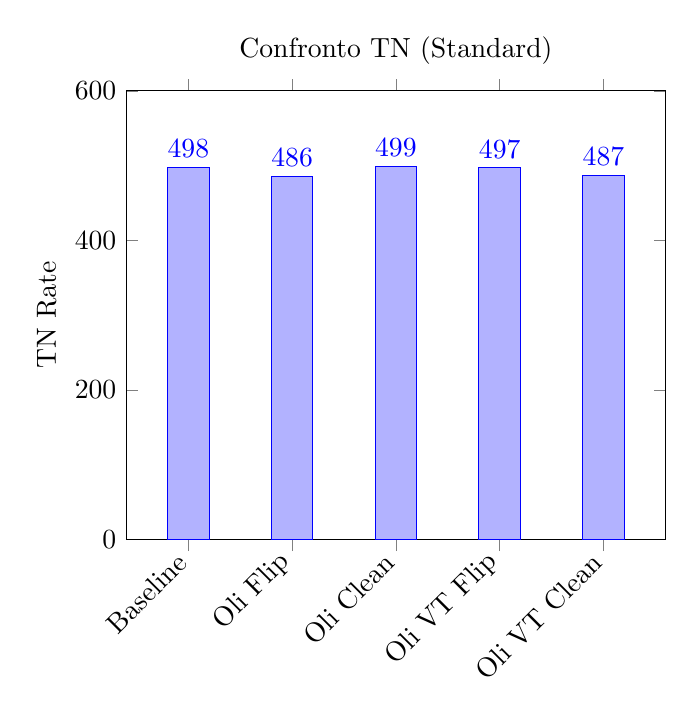
\begin{tikzpicture}
            \begin{axis}[
                ybar,
                symbolic x coords={Baseline, Oli Flip, Oli Clean, Oli VT Flip, Oli VT Clean},
                xtick=data,
                nodes near coords,
                ymin=0, ymax=600,
                ylabel={TN Rate},
                title={Confronto TN (Standard)},
                x tick label style={rotate=45, anchor=east},
                bar width=15pt,
                enlarge x limits=0.15
            ]
                \addplot coordinates {(Baseline,498) (Oli Flip,486) (Oli Clean,499) (Oli VT Flip,497) (Oli VT Clean,487)};
            \end{axis}
        \end{tikzpicture}
        }
        \caption{Confronto TN}
        \label{fig:tn_comparison_olivander_vt}
    \end{subfigure}
    \hfill
    \begin{subfigure}[b]{0.45\textwidth}
        \centering
        \resizebox{\textwidth}{!}{
        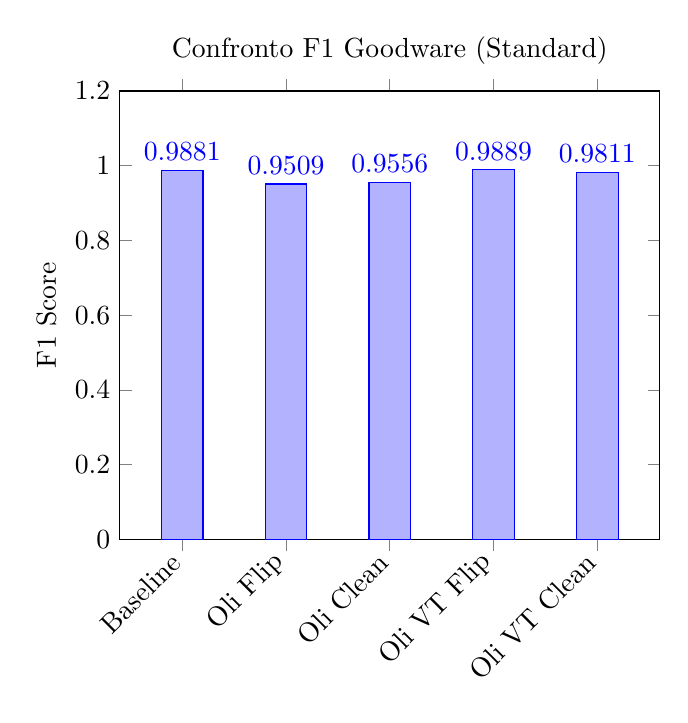
\begin{tikzpicture}
            \begin{axis}[
                ybar,
                symbolic x coords={Baseline, Oli Flip, Oli Clean, Oli VT Flip, Oli VT Clean},
                xtick=data,
                nodes near coords,
                nodes near coords style={/pgf/number format/.cd,fixed,precision=4,zerofill},
                ymin=0, ymax=1.2,
                ylabel={F1 Score},
                title={Confronto F1 Goodware (Standard)},
                x tick label style={rotate=45, anchor=east},
                bar width=15pt,
                enlarge x limits=0.15
            ]
                \addplot coordinates {(Baseline,0.9881) (Oli Flip,0.9509) (Oli Clean,0.9556) (Oli VT Flip,0.9889) (Oli VT Clean,0.9811)};
            \end{axis}
        \end{tikzpicture}
        }
        \caption{Confronto F1 Goodware}
        \label{fig:f1_goodware_comparison_olivander_vt}
    \end{subfigure}
    
    \vspace{1cm}
    
    \begin{subfigure}[b]{0.45\textwidth}
        \centering
        \resizebox{\textwidth}{!}{
        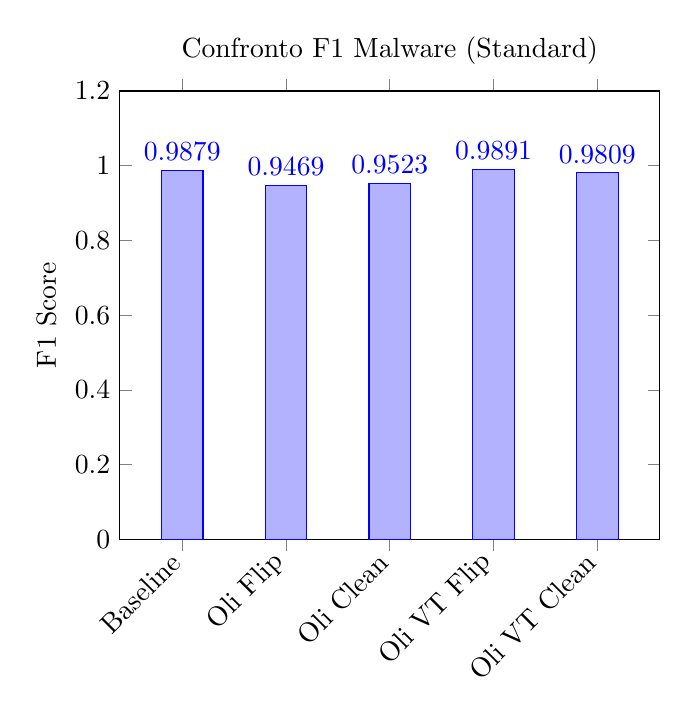
\begin{tikzpicture}
            \begin{axis}[
                ybar,
                symbolic x coords={Baseline, Oli Flip, Oli Clean, Oli VT Flip, Oli VT Clean},
                xtick=data,
                nodes near coords,
                nodes near coords style={/pgf/number format/.cd,fixed,precision=4,zerofill},
                ymin=0, ymax=1.2,
                ylabel={F1 Score},
                title={Confronto F1 Malware (Standard)},
                x tick label style={rotate=45, anchor=east},
                bar width=15pt,
                enlarge x limits=0.15
            ]
                \addplot coordinates {(Baseline,0.9879) (Oli Flip,0.9469) (Oli Clean,0.9523) (Oli VT Flip,0.9891) (Oli VT Clean,0.9809)};
            \end{axis}
        \end{tikzpicture}
        }
        \caption{Confronto F1 Malware}
        \label{fig:f1_malware_comparison_olivander_vt}
    \end{subfigure}
    \hfill
    \begin{subfigure}[b]{0.45\textwidth}
        \centering
        \resizebox{\textwidth}{!}{
        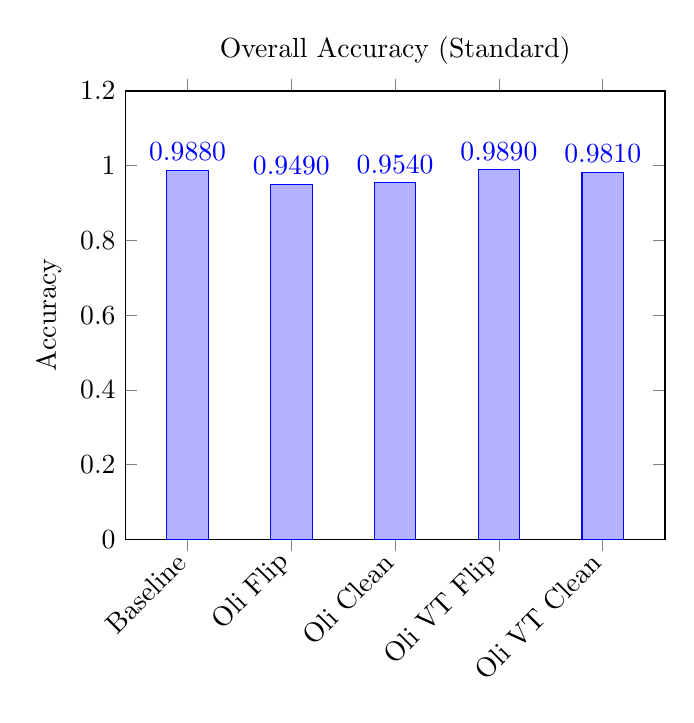
\begin{tikzpicture}
            \begin{axis}[
                ybar,
                symbolic x coords={Baseline, Oli Flip, Oli Clean, Oli VT Flip, Oli VT Clean},
                xtick=data,
                nodes near coords,
                nodes near coords style={/pgf/number format/.cd,fixed,precision=4,zerofill},
                ymin=0, ymax=1.2,
                ylabel={Accuracy},
                title={Overall Accuracy (Standard)},
                x tick label style={rotate=45, anchor=east},
                bar width=15pt,
                enlarge x limits=0.15
            ]
                \addplot coordinates {(Baseline,0.988) (Oli Flip,0.949) (Oli Clean,0.954) (Oli VT Flip,0.989) (Oli VT Clean,0.981)};
            \end{axis}
        \end{tikzpicture}
        }
        \caption{Overall Accuracy}
        \label{fig:accuracy_comparison_olivander_vt}
    \end{subfigure}
    \caption{Confronto metriche - OLIVANDER Standard vs VT Filtered}
    \label{fig:poisoning_olivander_vt_comparison}
\end{figure}

\begin{figure}[htbp]
    \centering
    \begin{subfigure}[b]{0.45\textwidth}
        \centering
        \resizebox{\textwidth}{!}{
        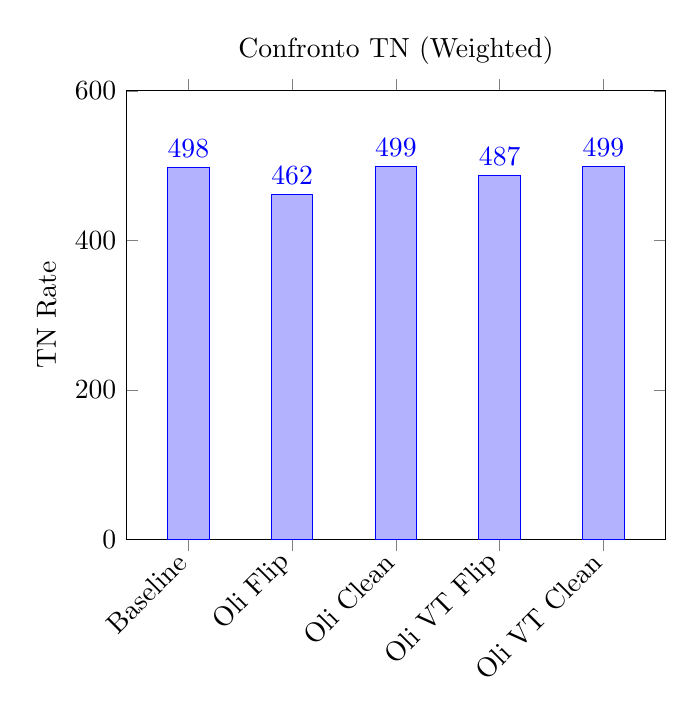
\begin{tikzpicture}
            \begin{axis}[
                ybar,
                symbolic x coords={Baseline, Oli Flip, Oli Clean, Oli VT Flip, Oli VT Clean},
                xtick=data,
                nodes near coords,
                ymin=0, ymax=600,
                ylabel={TN Rate},
                title={Confronto TN (Weighted)},
                x tick label style={rotate=45, anchor=east},
                bar width=15pt,
                enlarge x limits=0.15
            ]
                \addplot coordinates {(Baseline,498) (Oli Flip,462) (Oli Clean,499) (Oli VT Flip,487) (Oli VT Clean,499)};
            \end{axis}
        \end{tikzpicture}
        }
        \caption{Confronto TN}
        \label{fig:tn_comparison_olivander_vt_weighted}
    \end{subfigure}
    \hfill
    \begin{subfigure}[b]{0.45\textwidth}
        \centering
        \resizebox{\textwidth}{!}{
        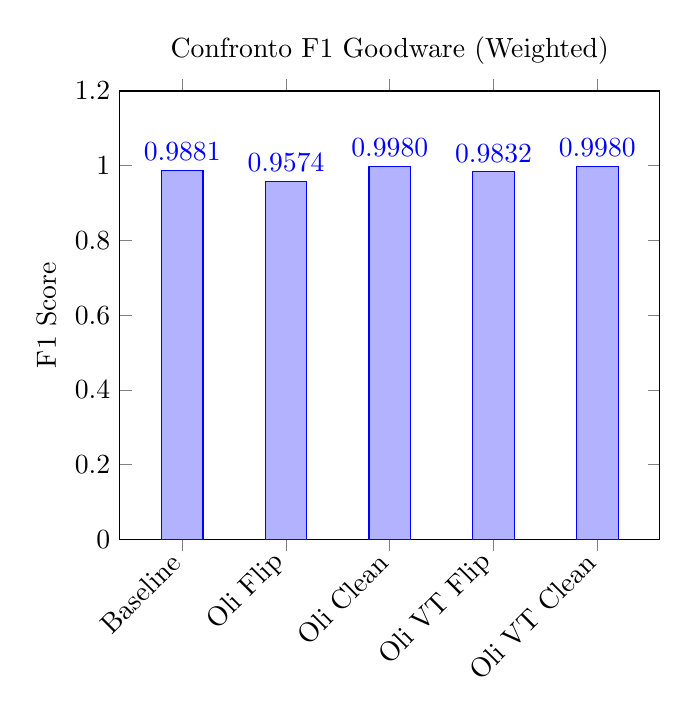
\begin{tikzpicture}
            \begin{axis}[
                ybar,
                symbolic x coords={Baseline, Oli Flip, Oli Clean, Oli VT Flip, Oli VT Clean},
                xtick=data,
                nodes near coords,
                nodes near coords style={/pgf/number format/.cd,fixed,precision=4,zerofill},
                ymin=0, ymax=1.2,
                ylabel={F1 Score},
                title={Confronto F1 Goodware (Weighted)},
                x tick label style={rotate=45, anchor=east},
                bar width=15pt,
                enlarge x limits=0.15
            ]
                \addplot coordinates {(Baseline,0.9881) (Oli Flip,0.9574) (Oli Clean,0.9980) (Oli VT Flip,0.9832) (Oli VT Clean,0.9980)};
            \end{axis}
        \end{tikzpicture}
        }
        \caption{Confronto F1 Goodware}
        \label{fig:f1_goodware_comparison_olivander_vt_weighted}
    \end{subfigure}
    
    \vspace{1cm}
    
    \begin{subfigure}[b]{0.45\textwidth}
        \centering
        \resizebox{\textwidth}{!}{
        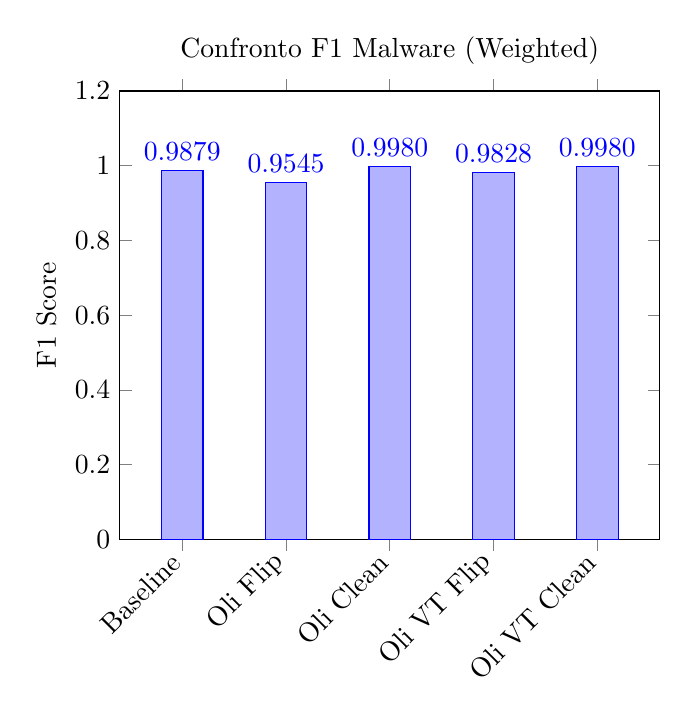
\begin{tikzpicture}
            \begin{axis}[
                ybar,
                symbolic x coords={Baseline, Oli Flip, Oli Clean, Oli VT Flip, Oli VT Clean},
                xtick=data,
                nodes near coords,
                nodes near coords style={/pgf/number format/.cd,fixed,precision=4,zerofill},
                ymin=0, ymax=1.2,
                ylabel={F1 Score},
                title={Confronto F1 Malware (Weighted)},
                x tick label style={rotate=45, anchor=east},
                bar width=15pt,
                enlarge x limits=0.15
            ]
                \addplot coordinates {(Baseline,0.9879) (Oli Flip,0.9545) (Oli Clean,0.998) (Oli VT Flip,0.9828) (Oli VT Clean,0.998)};
            \end{axis}
        \end{tikzpicture}
        }
        \caption{Confronto F1 Malware}
        \label{fig:f1_malware_comparison_olivander_vt_weighted}
    \end{subfigure}
    \hfill
    \begin{subfigure}[b]{0.45\textwidth}
        \centering
        \resizebox{\textwidth}{!}{
        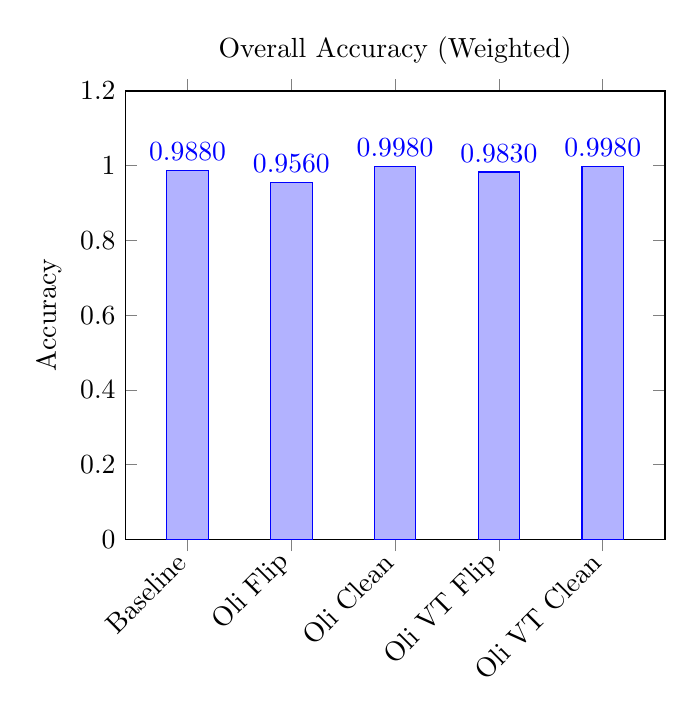
\begin{tikzpicture}
            \begin{axis}[
                ybar,
                symbolic x coords={Baseline, Oli Flip, Oli Clean, Oli VT Flip, Oli VT Clean},
                xtick=data,
                nodes near coords,
                nodes near coords style={/pgf/number format/.cd,fixed,precision=4,zerofill},
                ymin=0, ymax=1.2,
                ylabel={Accuracy},
                title={Overall Accuracy (Weighted)},
                x tick label style={rotate=45, anchor=east},
                bar width=15pt,
                enlarge x limits=0.15
            ]
                \addplot coordinates {(Baseline,0.988) (Oli Flip,0.956) (Oli Clean,0.9980) (Oli VT Flip,0.983) (Oli VT Clean,0.9980)};
            \end{axis}
        \end{tikzpicture}
        }
        \caption{Overall Accuracy}
        \label{fig:accuracy_comparison_olivander_vt_weighted}
    \end{subfigure}
    \caption{Confronto metriche - OLIVANDER Standard vs VT Filtered (Weighted)}
    \label{fig:poisoning_olivander_vt_comparison_weighted}
\end{figure}
